
\section{Introduction}\label{sec:introduction_4}

% Time series alignment methods, such as those presented in \cref{chapter:3} can be used as a preprocessing step before performing other machine learning tasks, such as clustering, classification, averaging, and so on. In this chapter one of these applications is discussed: \textbf{time series classification (TSC)}.

% \section{Time Series Classification}

% CLASSIFICATION
% Time series classification is one of the most appealing research domains in machine learning. The generality of interest is influenced by the large number of problems involving time series, ranging from financial econometrics up to medical diagnosis.

% Time series classification is the area of machine learning tasked with the categorization or labelling of time series.

% Time series classification is a branch of machine learning that deals with the analysis and classification of sequential data. This type of data is often found in various domains, such as finance, meteorology, and biology, and is characterized by its temporal dependencies and patterns.

% Time series classification problems arise in a wide range of fields including, but not limited to, data mining, statistics, machine learning, signal processing, environmental sciences, computational biology, image processing and chemometrics.


% APPLICATIONS
% Time series classification has been applied in many fields, with numerous organized open competitions and publicly available data sets. 
Applications of time series classification are diverse and include areas such as finance \cite{majumdar2020clustering}, power systems \cite{susto2018time}, healthcare \cite{wang2022multihead}, manufacturing \cite{hsu2021multiple} and environmental monitoring \cite{gundersen2020binary}. On the whole, time series classification is a powerful tool that provides valuable insights into patterns and trends in sequential data, and has the potential to significantly improve decision-making and outcomes in many fields. 
This article focuses on a specific industrial application: the \textbf{fault classification of hydraulic rock drill pressure data} under different configurations and scenarios, which was put forward by the Prognostics and Health Management Society \cite{phm} for the 2022 PHM Data Challenge\footnote{\url{https://data.phmsociety.org/2022-phm-conference-data-challenge/}}, an international open data competition specialized in industrial data analytics and covers a wide spectrum of real-world industrial problems. %In 2022, the competition consisted on a time series classification problem involving hydraulic rock drill pressure data, as was already mentioned.
% This chapter summarizes our participation in the 2022 data challenge. 
A novel solution was presented based on deep learning techniques that \textbf{simultaneously aligns and classifies faulty signals} with an accuracy of 97.80\%, ranking sixth out of 18 competitors.


This article is structured as follows.
Work related to time series classification is discussed in \cref{sec:related_work_4}. Then, the PHM challenge is described in \cref{sec:phm_challenge} and present the proposed model in \cref{sec:method_4}. Experimental results are included in \cref{sec:results_4} and final remarks are included in \cref{sec:conclusions_4}.

\clearpage

% RELATED WORK
\section{Related Work}\label{sec:related_work_4}

% TIME SERIES CLASSIFICATION
\textbf{Time series classification} is defined as the process of assigning a category to an unlabeled time series observation by exploiting patterns of the training data.
Let 
% $D=\{(X_{1}, y_{1}), (X_{2}, y_{2}), \ldots, (X_{n}, y_{n})\}$ 
$D=\{(X_{1}, y_{1}), \ldots, (X_{n}, y_{n})\}$ 
be a dataset containing a collection of pairs, where $X_{i}$ could either be a univariate or multivariate time series with its corresponding label denoted by $Y_{i}$.
Given such a set of $n$ labelled examples consisting of $d$ features measured at $T$ time steps ($X \in \mathbb{R}^{n \times T \times d}$), and the outcome labels $y \in \mathbb{R}^{n}$, the goal is to learn a mapping from $\{x_{t}^{(i)}\}_{t=1}^{T}$ to $y_{i}$ where $x_{t}^{(i)} \in \mathbb{R}^{d}$ and $i \in \{1,\cdots,n\}$ is an index into the $i^{th}$ sample. Each feature is represented as a set of $T$ measurements. 
Note that, in general, each time series can have a different number of observations $T$.


% [DUDA] Recent advancements in time series classification methods have improved the accuracy and efficiency of the predictions.
% Recent time series classification methods have made significant progress in improving the accuracy and efficiency of classification algorithms, enabling more accurate predictions and insights from time series data.
% STANDARD CLASSIFICATION METHODS
One of the key challenges in time series classification is to capture and model the \textbf{inherent temporal dependencies} and patterns in the data. Traditional machine learning algorithms, such as decision trees and support vector machines, are designed for cross-sectional data and are not suitable for TSC due to their inability to handle and harness the temporal information. 
For \textbf{traditional classification models} the order of the attributes is irrelevant and the interaction between variables is considered independent of their relative positions. For instance, the Naive Bayes algorithm assumes conditional independence between each feature given the label.
In contrast, for time series data, the ordering of the variables is crucial for identifying the best discriminating features, as the order of the values is an essential part of the time series, and consecutive time points are likely to be highly correlated. 

% METHODS THAT CAPTURE TEMPORAL DEPENDENCIES
To address this, \textbf{specialized time series algorithms} have been developed, such as dynamic time warping and recurrent neural networks, that are capable of capturing the temporal dependencies in the data. 
% Over the past few decades, there has been significant progress in the accuracy of time series classifiers. 
To compare different time series, specific metrics and kernels have been proposed \cite{abanda2019review}. Some algorithms involve extracting features from the time series data that can be fed into a standard machine learning classifier. Bag-of-words models that involve discretizing the time series are popular, with many algorithms being developed for this approach. Other algorithms work directly on raw time series data, as the one proposed in \cref{sec:method_4}. Transforming time series data into images has also been studied as a potential preprocessing method for classification. 
This section presents a review of current approaches for time series classification.

% Standard machine learning classification algorithms, which are designed for structured data, are not always well suited for unstructured data such as time series. 
% Time series classification differs significantly to traditional supervised learning for structured data, in that the algorithms should be able to handle and harness the temporal information present in the signal. 

% https://arxiv.org/pdf/1909.04939.pdf


\subsection{$k$ Nearest-Neighbor Methods}

Nearest-neighbor methods are based on the notion of similarity, and the prediction of a new sample is made based on the target value of $k$ similar samples.
Consequently, the key element of nearest-neighbor algorithms is the metric that defines the \textbf{similarity between any pair of samples}.
The choice of distance measure is dependent on the domain and, more specifically, the invariances required by the domain. 
% In light of this, numerous techniques have been designed to efficiently measure the similarity between time series with invariance to various combinations of amplitude scaling, offset, local warping, uniform scaling, phase, occlusion or noise (see \cref{sec:invariances}).

% The prediction for a new sample is based on the target value of similar samples. A key element of nearest-neighbor algorithms is the metric, that is, the mathematical function defining the similarity between any pair of samples.
% This type of classifiers compares two series using a certain distance. 

The classic benchmark for TSC has been the nearest neighbor algorithm coupled with the Dynamic Time Warping similarity measure (NN-DTW) \cite{bagnall2017great}, while NN with Euclidean distance was fairly easy to beat.  Elastic measures, such as DTW, are intended to compensate for local distortions, misalignments, or warpings in time series caused by stretched or shrunken sections. It should be noted, however, that NN-DTW is highly sensitive to noise in the training set, which is a strong trait of time series datasets \cite{abanda2019review}.
Much research has focused on finding alternative efficient similarity measures. Commonly used similarity measures include variations of DTW such as TWED \cite{marteau2008time}, SoftDTW \cite{cuturi2017soft}, DDTW \cite{keogh2001derivative} and others SBD \cite{paparrizos2017fast}, LCSS \cite{vlachos2002discovering}, or GAK \cite{cuturi2011fast}. A comprehensive review of distance-based time series classification methods can be found in \cite{abanda2019review}. 

Ensembles formed by combining multiple 1-NN classifiers with diverse similarity measures have proven to be considerably more accurate than 1-NN with any single measure \cite{bagnall2015time}. Such ensembles aid in reducing model variance and thus improving overall classification accuracy. 
For example, Elastic Ensemble \cite{bagnall2015time} combines eleven 1-NN algorithms, each using a different elastic measure.

% \cite{stefan2012move}, \cite{keogh2001derivative}

% Another research area focused on proposing global alignment kernels such as SoftDTW introduced by Cuturi and Blondel (2017), that can be further used in a nearest centroid classification scheme. 
% There is a wide range of classification algorithms that can be used for time series analysis. 
% Current empirical evidence suggests that the nearest-neighbor methods are difficult to beat. 


\subsection{Tree-based Algorithms}


Tree-based machine learning algorithms, such as random forest \cite{breiman2001random}, build a tree-like structure in which each internal \textbf{node represents a decision based on certain features} of the data, and each leaf node represents a final prediction. In TSC, these algorithms are applied to the time series data by segmenting it and extracting features from each segment to feed the decision tree.

% have proven to be powerful and effective. 
Time Series Forest \cite{deng2013time} considers subsequences generated from random start and end indices, based on a minimum length for the interval, which is a hyperparameter. From these intervals, Time Series Forest applies three time domain transformations (mean, standard deviation and slope), and then trains a decision tree using these features. The operation is repeated to learn an ensemble of decision trees, similar to Random Trees, on different randomly chosen intervals.
Time Series Bag-Of-Features \cite{baydogan2013bag} extracts more features than Time Series Forest. Each randomly sampled interval is divided into non-overlapping subintervals, and four features are extracted: mean, standard deviation, as well as the start and end indices of each subinterval.

The Proximity Forest algorithm \cite{lucas2019proximity} works directly with raw time series to  build an ensemble of classification trees in which data at each node is split based on similarity to a representative time series from each class. This differs from the typical attribute-value splitting methods used in decision trees.
In a similar vein, TS-CHIEF \cite{shifaz2020ts} is a stochastic tree-based ensemble designed for speed and high accuracy, where at each node the algorithm selects from a random selection of TSC methods the one that best classifies the data reaching that node.


\subsection{Dictionary-based Algorithms}

Dictionary-based algorithms provide an efficient way to handle time series data by transforming it into a bag of words representation. These techniques are particularly adept at addressing noisy data and recognizing repeating patterns. To achieve this, the series is first shortened using an approximation method, and then a quantization method is used to discretize the values, thereby forming words. Each time series is represented by a histogram that counts words frequency. Notable dictionary based algorithms are BOP \cite{lin2012rotation}, SAX \cite{lin2003symbolic}, SAX-VSM \cite{senin2013sax}, SFA \cite{schafer2012sfa} and BOSS \cite{schafer2015boss}. 


% \subsection{Shapelet-based Techniques}




\subsection{Imaging Time Series}



Several methods have been proposed for transforming time series (vectors) into images (matrices). 
The \textbf{recurrence plot} \cite{eckmann1995recurrence} is a matrix consisting of the binarized pairwise distances between all the pairs of trajectories (a subsequence of equally spaced values) from a time series. Visually, as a black-and-white image, a pixel is black if and only if the distance between the two considered trajectories is smaller than the threshold.

Also related, the \textbf{Gramian angular field} \cite{wang2015encoding} is based on the polar coordinate representation of time series and measures the temporal correlation by computing the trigonometric sum or difference between all the pairs of angles. Gramian angular fields have been used for time series classification as a preprocessing step to generate images used as input of a tiled convolutional neural network.

\textbf{Markov transition field} \cite{wang2015encoding} assumes after discretization that a time series is a Markov chain. First, a time series of length $n$ is discretized based on its quantile bins $Q$. Second, by considering this discretize-valued time series as observations of a first-order Markov chain, one can compute the number of occurrences of pairs of back-to-back bins for every pair of bins. This matrix is then normalized to transform the frequencies into probabilities, leading to the Markov transition matrix. The Markov transition matrix is insensitive to the temporal distribution of the time series since it only captures the frequencies of the transition, but not at which time points they occurred. Moreover, its size depends on the number of bins and not the length of the time series. To overcome these issues, the Markov transition matrix is projected onto a $n \times n$ matrix that is called the Markov transition field. Like Gramian angular fields, Markov transition fields have been used for time series classification as a preprocessing step to generate images then train a tiled convolutional neural network. 

\begin{figure}[!htb]
    \begin{center}
        \begin{subfigure}[b]{0.315\linewidth}
            \centering
            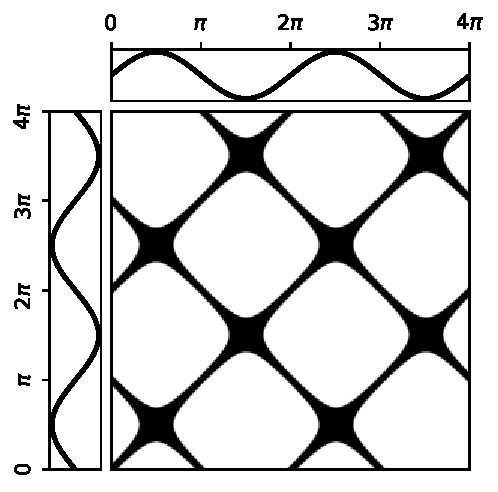
\includegraphics[width=\linewidth]{figures/imaging_1.pdf}
            \caption{Recurrence Plot}
        \end{subfigure}
        \hfill
        \begin{subfigure}[b]{0.32\linewidth}
            \centering
            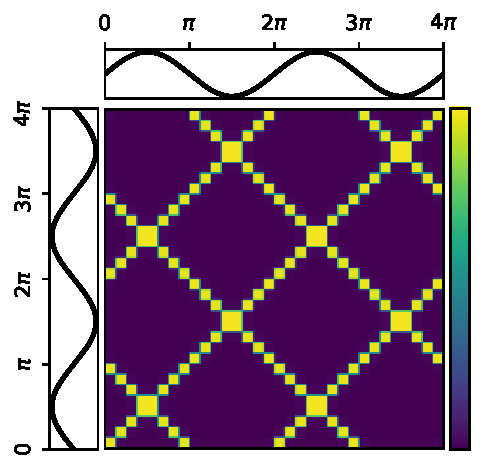
\includegraphics[width=\linewidth]{figures/imaging_2.pdf}
            \caption{Markov Transition Field}
        \end{subfigure}
        \hfill
        \begin{subfigure}[b]{0.32\linewidth}
            \centering
            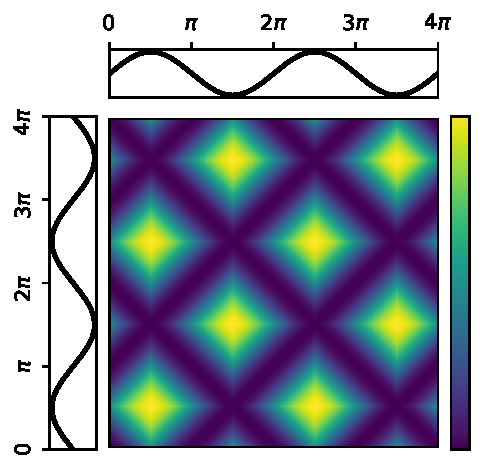
\includegraphics[width=\linewidth]{figures/imaging_3.pdf}
            \caption{Gramian Angular Summation}
        \end{subfigure}
        \hfill
        \caption{Time series imaging example with a sine function in the interval $[0,4\pi]$. \textbf{Left}: the recurrence plot uses a threshold value of $0.1$. \textbf{Center}: the Markov transition field shows that the sine function is periodic with period $2\pi$ and smooth. \textbf{Right}: Gramnian angular summation field}
    \label{fig:imaging_ts}
    \end{center}
\end{figure}

% IMAGE CLASSIFICATION VS TIME SERIES CLASSIFICATION
\begin{remark}
    This scenario has obvious similarities with computer vision tasks like image classification and object localization, where deep learning algorithms can learn from the spatial information contained within an image. TSC is in essence a similar problem, but with one less dimension. Despite this resemblance, the state-of-the-art algorithms in the two fields have little in common.
\end{remark}
    

\subsection{Deep Learning}

Over the past decade, deep learning has led to many breakthroughs in several fields such as computer vision \cite{fawaz2019deep} and natural language processing \cite{floridi2020gpt}. Deep learning has also been recently investigated for time series classification.
\textbf{Convolutional Neural Networks} (CNNs) have showed promising results for TSC \cite{wang2017time}. Given an input multivariate time series, a convolutional layer consists of sliding one-dimensional filters over the time series, thus enabling the network to extract non-linear discriminant features that are time-invariant and useful for classification. By cascading multiple layers, the network is able to further extract hierarchical features that should in theory improve the network's prediction. 

% Time LeNet
In this sense, Fully Convolutional Neural Networks (FCNs) \cite{wang2017time} were shown to achieve great performance without the need to add pooling layers to reduce the input data's dimensionality. 
% ResNet can further improve the classification performance
\textbf{InceptionTime} \cite{fawaz2019deep} is an ensemble of 60 neural network models to perform time series classification. The 60 models come from 6 architectures: a multi-layer perceptron, a fully convolutional neural network, a residual network, an encoder, a multi-channel deep convolutional neural network and a time convolutional neural network.

% \subsection{Random Convolutions}
CNNs have a large number of trainable parameters in comparison to more classic algorithms such as logistic regression or support vector machines, thus usually requiring a large sample size to find good values for the trainable parameters. Based on this observation, the \textbf{Random Convolutional Kernel Transform} (ROCKET) \cite{dempster2020rocket} extracts features from time series using a large number of random convolutional kernels, meaning that all the parameters of all the kernels (length, weights, bias, dilation, and padding) are randomly generated from fixed distributions. 
% Instead of extracting a single feature for each kernel, such as the maximum or the mean, as it is usually performed in convolutional neural networks, two features are extracted: the maximum and the proportion of positive values. 
The classifier built on top of the transformation is then responsible for selecting the most relevant features to perform classification. It has a much lower computational complexity than the best-performing time series classification algorithms while having a comparable performance.


% CONVOLUTIONS
\begin{remark}
    Applied to time series data, 1D convolutions inherently capture phase invariance and noise invariance, to a degree.
    % In particular, CNNs are capable of efficiently handling phase invariance and noise invariance, to a degree.
    % (i.e., the use of a filter slid along the temporal dimension allows for variability in the starting point of temporal patterns.) 
    % CNNs also handle noise invariance, to a degree. 
    Max pooling coupled with multiple layers allows the model to smooth the inputs and learn higher-level abstractions.
    However, temporal invariances such as warping must also be considered. Data may be collected from different sources, at different times, and using different sampling frequencies, which may lead to misleading results.
    % , in addition to magnitude and offset invariances. %Due to the inherent differences between these types of invariances, we address them separately in the two subsections that follow.
\end{remark}
    


\subsection{Ensemble Models}

Ensemble-based methods combine different classifiers together to achieve a higher accuracy. For example, Collective of Transformation-Based Ensembles (COTE) \cite{bagnall2015time} uses an ensemble of different classifiers over different time series representations.
Hierarchical Vote Collective of Transformation-Based Ensembles (HIVE-COTE) \cite{lines2018time} is an extension of COTE with a new type of spectral classifier called Random Interval Spectral Ensemble, two more classifiers (BOSS \cite{schafer2015boss} and Time Series Forest \cite{deng2013time}) and a hierarchical voting scheme, which further improves the decision taken by the ensemble.
HIVE-COTE recognizes time series data as a distinct data type for which the traditional attribute-value representation, which is commonly used in machine learning, does not provide a suitable representation.
In terms of classification accuracy, HIVE-COTE is the current state of the art, but it is often infeasible to run on even modest amounts of data. 

% HIVE-COTE combines multiple types of classifiers: each extracting information about a specific aspect of a time series, be it in the time domain, frequency domain or summarization of intervals within the series. However, HIVE-COTE (and its predecessor, FLAT-COTE) is often infeasible to run on even modest amounts of data. 

% Time Series Combination of Heterogeneous and Integrated Embedding Forest (TS-CHIEF): builds a random forest of decision trees whose splitting functions are time series specific and based on similarity measures, dictionary (bag-of-words) representations, and interval-based transformations. rivaling with HIVE-COTE in terms of predictive performance while having a substantially lower run time.



% \section{Time Series Averaging}
% Fréchet mean formulation that allows computing barycenters under the new geometry (after alignment)




\section{Rock Drill Fault Detection: PHM Challenge}\label{sec:phm_challenge}


The 2022 PHM challenge \cite{phm} addresses the problem of \textbf{fault classification for a rock drill} application under different individual configurations of the rock drill. The task is to develop a fault diagnosis model using the provided pressure sensor data as input. 
The application of TSC methods for fault classification holds significant potential for various industries, including the hydraulics sector within the mining industry. The drive towards automation and remote operation in the mining industry is motivated by the desire to create a safer working environment by reducing human presence near machines and hazardous work areas \cite{jakobsson2022time}.

\subsection{Industrial Application}

% % 1. Introduction
% \subsection{Introduction to the Industrial Problem}

Hydraulic rock drills are used in a wide range of applications where holes are needed in hard rock materials. Such systems, as seen in \cref{fig:phm_1}, often operate under high performance demands in harsh environments, with vibrations and moisture. 
% Normally no high resolution measurement data is available from such machines, and especially not in combination with known internal faults. 
% Any sensor must be robust and reliable, leading to high costs and minimizing the number of sensors is of importance. 
For this work, data is measured using a single pressure sensor located on the inlet pressure line where many effects of internal conditions are believed to manifest. 


\begin{figure}[!b]
    \begin{center}
        \begin{subfigure}[t]{0.38\linewidth}
        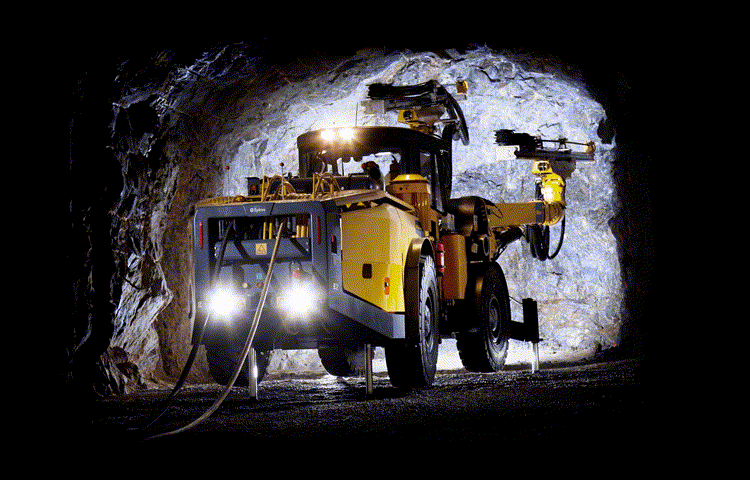
\includegraphics[width=\linewidth, trim=80 80 80 20, clip]{figures/drill_1_min.png}
        \caption{Rock drills on a drill rig in their natural underground habitat. 
        % Asset: Epiroc. 
        % The rock drill consists of four main systems. The percussion system, where an impact piston is caused to oscillate by use of hydraulic fluid power. The rotation system, where a hydraulic motor rotates the drill steel. The damper system, where stress wave reflections from the rock are dissipated as heat, and the flushing system, where flushing media enters the drill steel.
        The rock drill is composed of four primary systems: percussion, rotation, damper and flushing. This work primarily targets the percussion and damping system.
        % The rock drill is composed of four primary systems. In the \textbf{percussion} system, a hydraulic fluid drives an impact piston to oscillate. In the \textbf{rotation} system, the drill steel is rotated by a hydraulic motor. The \textbf{damper} system dissipates stress wave reflections from the rock as heat, and the \textbf{flushing} system, where flushing media enters the drill steel.
        }
        \label{fig:phm_1}
    \end{subfigure}
    \hfill
    \begin{subfigure}[t]{0.6\linewidth}
        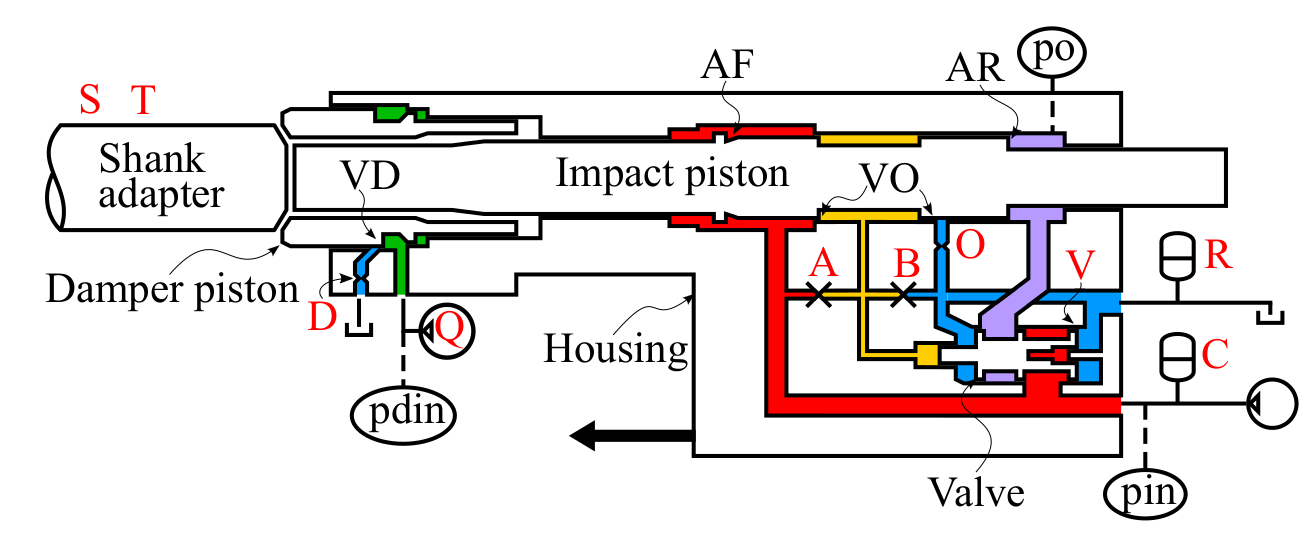
\includegraphics[width=\linewidth]{figures/drill_3.png}
        \caption{Diagram of the percussion and damper system, with 10 induced fault modes in red capital letters, and sensor locations (\textit{pin, po, pdin}) in ovals. Colored areas represent various hydraulic lines such as \textcolor{red}{high pressure supply} (red), \textcolor{blue}{low pressure return} (blue), \textcolor{violet}{alternating pressure} (purple), \textcolor{ForestGreen}{damper pressure} (green) and \textcolor{orange}{control pressure for the valve} (yellow).}
        \label{fig:phm_3}
    \end{subfigure}
    \caption{Rock drill information. Adapted with permission from \cite{jakobsson2022dataset}.}
    \label{fig:phm_1_3}
  \end{center}
\end{figure}


% A hydraulic rock drill, as seen mounted on an underground drill rig in \cref{fig:phm_1}, is a hydromechanical device using for generating stress waves in a drill steel. The rock drill is attached on a sliding cradle at the rear of a beam on the rig. The drill rig positions the beam and supplies the rock drill with hydraulic oil, flushing fluid, feed force and compressed air.

% The generated stress waves are transferred through a drill rod to a drill bit where tungsten carbide button bits crushes rock and creates a hole, typically around 30-60 mm in diameter for this type of machine. The drill bit is caused to rotate to allow new uncrushed rock in front of the button bits before the next impact occurs. Some flushing media, air or water, is flushed through the drill steel and bit to remove the debris.

% The rock drill consists of four main systems. The percussion system, where an impact piston is caused to oscillate by use of hydraulic fluid power. The rotation system, where a hydraulic motor rotates the drill steel. The damper system, where stress wave reflections from the rock are dissipated as heat, and the flushing system, where flushing media enters the drill steel. This work primarily targets the percussion- and damping system. A schematic image of these two systems are seen in \cref{fig:phm_3}.


A hydraulic rock drill is a hydromechanical device using for generating stress waves in a drill steel (see \cref{fig:phm_3}). It operates at frequencies where oscillations from \textbf{pressure propagation} is a phenomenon that needs to be taken into account. 
This causes small external changes that are not faults, such as changes in hose lengths, to significantly alter the behavior of the pressure signals. To capture such differences, different individuals are tested and included in the data. 
% To introduce such individual differences typically requires changing a number of parts physically in the test setup. 
% Further properties of the application include: 
Furthermore, the measured signal is periodic, and governed by some cyclic phenomenon such as the repeated opening of a valve. It has strong non-linearities, produced by impacts and sudden valve openings. The fundamental machine frequency is influenced by various disturbances, causing different events to occur at different times during a cycle depending on faults and individual variation such as unit configuration and manufacturing tolerances.
% There is wave propagation phenomenon, and since different events vary in time, it is difficult to predict how the superposition of the pressure waves occur.

% ALIGN DATA
Such complex temporal dynamics produce time series data that is not directly comparable, making it difficult for TSC methods to accurately classify the data. In order for these techniques to be effective, time series data must be consistently aligned. The model proposed in \cref{sec:method_4} automatically handles these temporal dependencies in the data using an extension of the Temporal Transformer Network presented in \cite{martinez2022closed}.

% \textcolor{red}{TO-DO}
% One of the key challenges in aligning time series data is the fact that the data may be collected from different sources, at different times, and using different sampling frequencies. This can result in time series data that is not directly comparable, which can make it difficult to accurately classify the data.

% In order for these techniques to be effective, it is necessary to align the time series data in a consistent manner. This alignment is important because it allows the data points to be compared and analyzed in a meaningful way. Without alignment, the data points may be misinterpreted or misclassified, leading to inaccurate or misleading results.



% Time series classification methods have potential to be used for fault classification from measurement data in many applications, including the application studied here, hydraulics in the mining sector. Automation and remote operation are trends driven by the desire to make mines safer by moving people away from machines and hazardous working environments. A logical side effect from this is a reduced awareness for operators and service personnel regarding the machines operating condition \cite{jakobsson2022time}. % https://arxiv.org/pdf/2203.16121.pdf

\subsection{Nature of Data}

% Data is collected in a series of test-cell experiments with introduced faults and pre-defined individual variations. The measurement setup allows for some easily changed parameters such as pressures and flows. This makes it possible to do full factor trials for such parameters, and many such combinations are available in the data set.  

The data set provides \textbf{normalized pressure measurements} from a hydraulic rock drill, operating in a close-to-reality type of test cell, while different faults and other  pre-defined variations are introduced to the system in a controlled manner. 
% The data is normalized and divided into separate impact cycles.
% The number of combinations required, together with the different faults induced, quickly add up to a large number of disassembly/assembly operations. It is also difficult to foresee all differences that may occur for combinations of part tolerances and drill rig configurations in the field. To overcome these problems and to reduce manual labor, control parameters are used as replacement for physical changes to emulate individual differences. 

There are 11 different \textbf{fault classification categories} (see \cref{tab:faults}), in which 10 are different failure modes and one class is from the healthy/no fault condition. 
The approximate location in the rock drill where faults are introduced are shown in red capital letters in \cref{fig:phm_3}. %The different classes are listed in Table 2 where the Letter column corresponds to the fault location seen in \cref{fig:phm_3}. The Label corresponds to the class labels used in the first column of the supplied data files. 
The differences between some fault classes are small compared to the individual differences, making this a challenging classification task.


\begin{table}[!htb]
    \small
    \caption{Fault classification categories}
    \label{tab:faults}
    \vspace{-1em}
    \begin{center}    
    \begin{tabular}{lll}   
        \toprule 
        Label & Letter & Description \\
        \midrule
        1 & NF & No-Fault \\
        2 & T & Thicker drill steel. \\
        3 & A & A-seal missing. Leakage from high pressure channel to control channel. \\
        4 & B & B-seal missing. Leakage from control channel to return channel. \\
        5 & R & Return accumulator, damaged. \\
        6 & S & Longer drill steel. \\
        7 & D & Damper orifice is larger than usual. \\
        8 & Q & Low flow to the damper circuit. \\
        9 & V & Valve damage. A small wear-flat on one of the valve lands. \\
        10 & O & Orifice on control line outlet larger than usual. \\
        11 & C & Charge level in high pressure accumulator is low. \\
        \bottomrule
    \end{tabular}
    \end{center}
\end{table}

\paragraph{Reference Data}
Furthermore, data from multiple individuals is scarce and does not cover the expected variability upon deployment. 
% However, a key requirement for a condition monitoring application is the availability of few nominal measurements from each individual upon deployment. 
As a result, organizers provide reference data from each individual upon deployment. %that may improve classification results. %from measurement data with a large impact from wave propagation.
The challenge is to create models able to generalize over individuals, while having access to some reference data from the specific individual. 
% Hence, it is important to use different individuals in training and validation. 
%The reference data from the validation individual can be considered unknown until a fictive deployment of the method. Hence this validation data can not be used during training.


\paragraph{Data Collection}

% A picture from the actual test setup is seen in \cref{fig:phm_4}. 
%Pressure measurements on three different locations are listed in Table 1, however the specific model and make of sensors and data acquisition equipment is left undisclosed due to proprietary reasons. 
% The test cell control system allows for automatic test sequences, including set levels of pressures, forces and flows. This functionality is used to emulate the individual differences expected to be found in a large population of rock drills and drill rigs.

For each case, ten seconds of data is collected, corresponding to approximately 800 impact cycles sampled at 50kHz. The ten second long time series are divided into shorter segments, containing one impact cycle each. 
% This split is done at the time of impact to capture the main stochastic element of the data generation. %, the response from hitting the shank adapter and possible reflections from the rock affecting the return velocity of the piston.
% The data set contains 11 different classes, including the No-fault class which also serves as reference. 
The automated collection sequence is shown in \cref{fig:phm_5}, where two configuration variables percussion pressure (P1) and feed force (P2) are changed according to the graph. %, in the same order for each class. The times of collection for the individuals are shown by the numbered intervals.
Note that P2 has a larger influence on the pressure signature than P1, so it is easier to generalize between certain classes.
% To expand the useful data two controlled variables, percussion pressure and feed force, are chosen as alternatives to real individuals such as different rock drills or drill rig types. By doing so, a larger number of combinations between individuals and fault types can be investigated with the available data set.
% Most of the induced faults requires disassembly of the rock drill, such as removing seals, orifices and exchanging parts. The following sequence is used for each fault:
% 1. Disassemble the rock drill. 2. Change / remove / modify parts to induce the different faults. 3. Assemble rock drill. 4. Run test cycle according to \cref{fig:phm_5}. The variation of parameters in the cycle gives data for different individuals. 5. Save data for the different individuals.
The structure of the data is shown in \cref{fig:phm_6}. In total 8 individuals $\times$ 11 classes $\times$ 300 to 700 cycles each give approximately 54000 cycles in total, each with data from 3 sensors. Each pressure time series range from 556 to 748 samples. The size of the dataset in $.csv$ format is 976 MB. 


\paragraph{Train / Test / Validation Split}
The training set consists of data from various faults from five individual configurations, while the test data is from one individual setup of the rock drill. The validation set for the final scoring for the competition is from two individual configurations from the rock drill and the labels were blind to the contest participants. For both the test and validation sets a reference from a No-Fault health condition is provided.

% The data is intended to be used in the following way: 1. Training data is supplied from a number of individuals. Reference data describing the No-fault case is also available. 2. Models are trained using the data. 3. Unseen data is presented from new individuals. Together with this unseen, possibly faulty data, there are a comparably small amount of reference measurements from the No-fault class from each specific individual. 4. The target is to classify the unseen data.






\begin{figure}[!htb]
    \begin{center}
        \begin{subfigure}[t]{0.46\linewidth}
        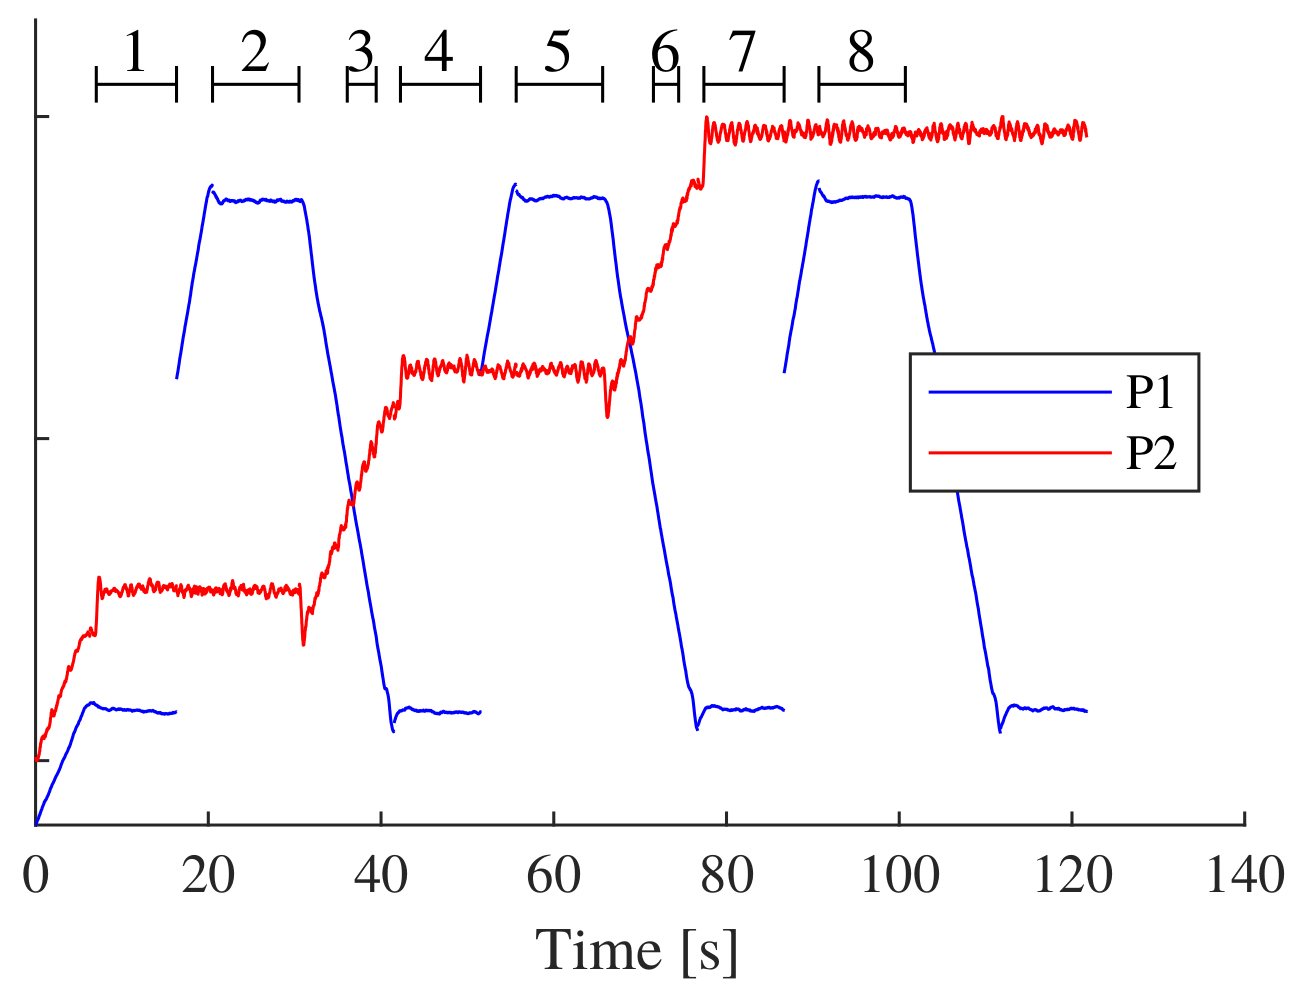
\includegraphics[width=\linewidth]{figures/drill_5.png}
        \caption{To simulate different individual configurations, the percussion pressure (P1) and feed force (P2) are changed. Markers in black show where individuals 1 through 8 are collected.}
        \label{fig:phm_5}
    \end{subfigure}
    \hfill
    \begin{subfigure}[t]{0.51\linewidth}
        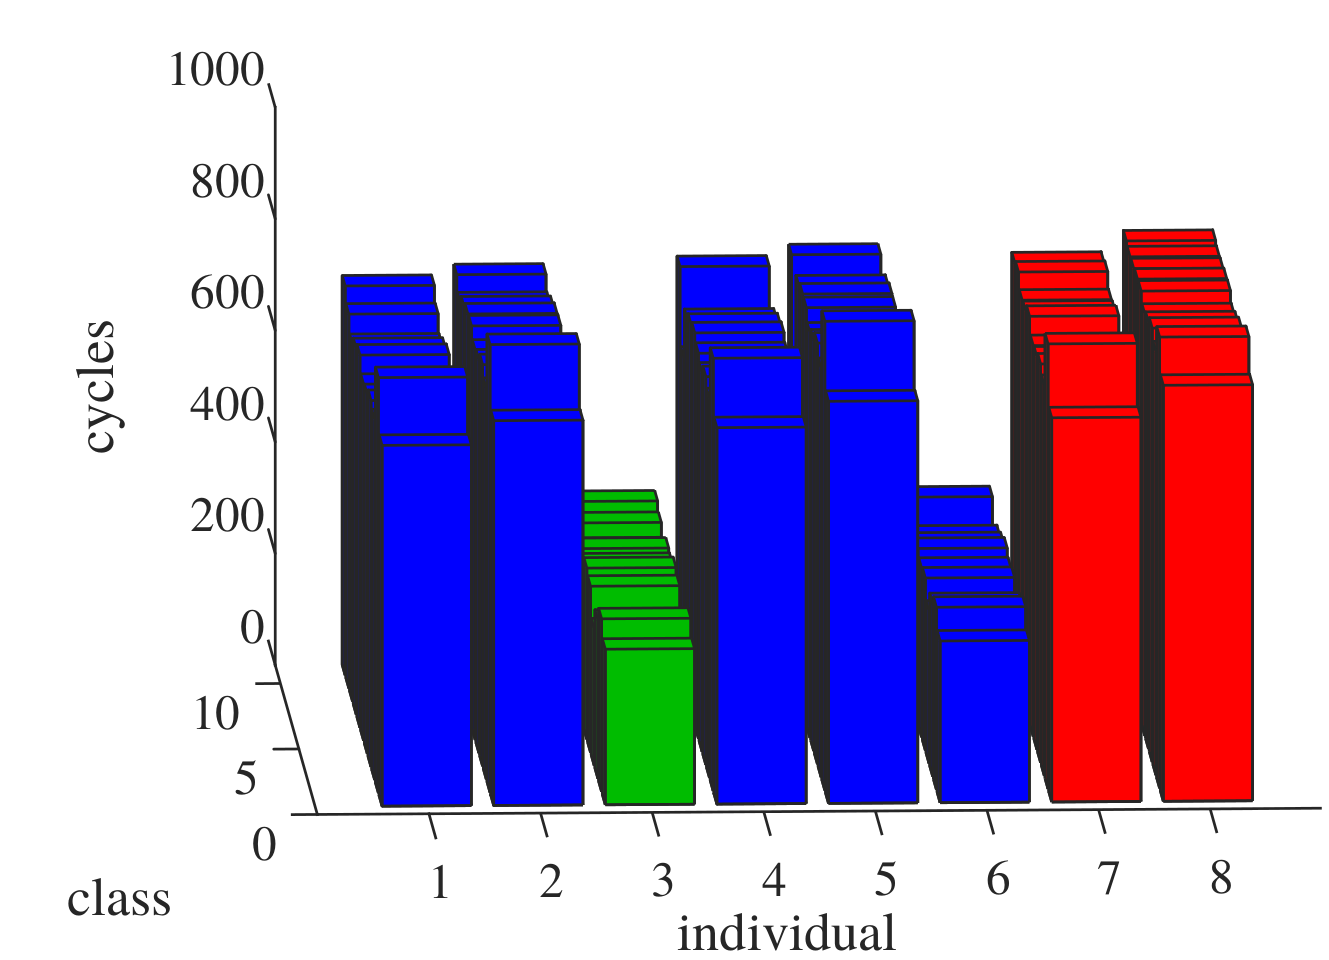
\includegraphics[width=\linewidth]{figures/drill_6.png}
        \caption{Number of cycles for each class and individual. Blue represents training data, green is data used for online scoring (test set) and red a holdout test set used for official competition scoring (validation).}
        \label{fig:phm_6}
    \end{subfigure}
    \caption{Data collection stats. Adapted with permission from \cite{jakobsson2022dataset}.}
    \label{fig:phm_5_6}
  \end{center}
  \end{figure}





% This work intends to discuss some particularities of how to approach an application, where training data from different individuals is scarce and does not cover the variability expected upon deployment.
% A key prerequisite is the availability of a small amount of nominal measurements from each individual upon deployment, a reasonable assumption for a condition monitoring application. The contribution of this work is a method how to use this reference data to improve classification from measurement data with a large impact from wave propagation.


% DATASET


% The task is to train a model to classify the fault conditions using the training data, and to test this model on the testing data, in which the one submission per day can be used for submitting results to the online leaderboard. Validation is done with a validation data set that will be released for a one-time assessment at the end of the data challenge. Scoring of performance is done through this web interface.

% The top three teams will be asked to submit their approach as a journal paper to the International Journal of Prognostics and Health Management (IJPHM) and present their approach and results at the 2022 PHM Society Conference. Top teams are also being recognized at the banquet and will receive a plaque. The official scoring for the competition is based solely on the validation data set.



% Problems with individual differences
\paragraph{Individual Differences}


% take into account individual differences when evaluating detection performance. 


Two individuals can have quite different pressure signatures due to a difference in supply hose length. \cref{fig:phm_2} shows an example of how individual differences can confound the pressure trace in a fault scenario compared with a No-Fault (NF) case. 
In fact, the oscillation seen around $t = 9$ arrives later as the fault is introduced, but this disparity can be masked by individual differences. A known reference from the current individual might be required for calibration \cite{jakobsson2022time}. % https://arxiv.org/pdf/2203.16121.pdf

% The zoomed section at t = 9 ms shows how an oscillation in time series $x_A^1$ starts to lag behind the reference. This is true also for the second individual, but would be very difficult to see without comparing to the second individuals reference case x2NF. If only x1A was part of the training data, it would thus be difficult to classify an unseen example from x2A. This poses a problem, since reference data for classification will originate from one or a few different individuals only.

To address this issue various strategies can be employed. The machine learning approach is to collect enough fault data from multiple individuals to train a model that can generalize well for unseen variations. Another approach is to build a physics-based model rooted on fundamental principles and refine it using data obtained from specific individuals. This method, although effective, can be both costly and time-consuming, particularly for complex systems. 
A third strategy is to gather limited data from few individuals and then personalize the model to suit specific individuals. The model in \cref{sec:method_4} adopts this approach. 

% Different strategies can be used to address this issue. Either, one collects sufficient fault data from different faults in different individuals to find a model capable of generalizing sufficiently for unseen variations.  This is the common machine learning approach. An alternative path is to build a physics based model based on first principles, and adapt it using data from specific individuals. For complex systems, such modeling can be both expensive and time-consuming, if even possible. A third approach lies somewhere between the first two, to collect a limited set of data from just a few individuals, and then to adapt this model to specific individuals. Our proposed model follows this third approach.



\begin{figure}[!htb]
    \begin{center}
    \centerline{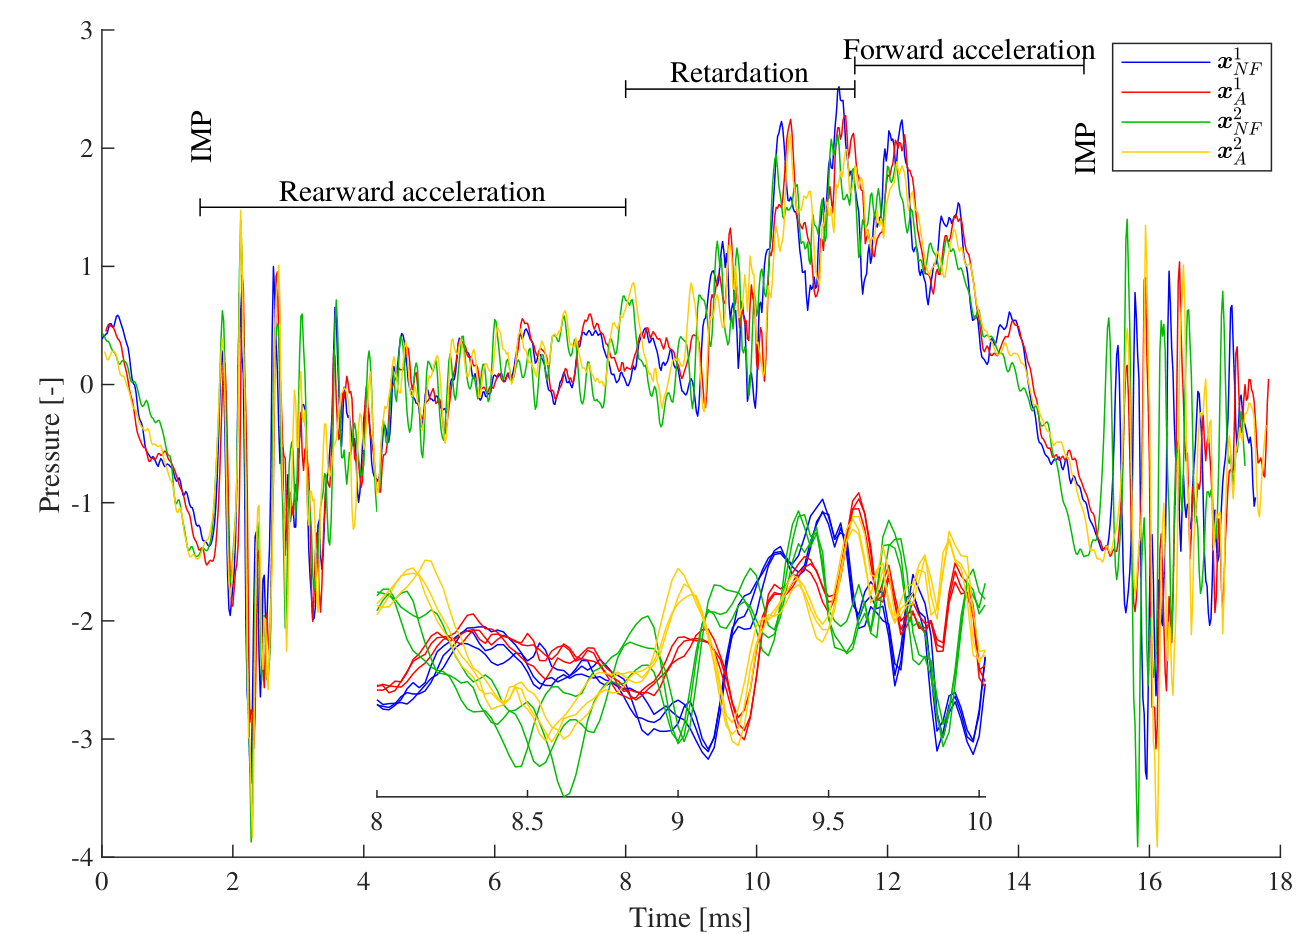
\includegraphics[width=0.9\linewidth]{figures/drill_2.png}}
    \caption{Pressure from two classes (NF and A), and two individuals (1 and 2). 
    % Multiple cycles are included to show the deterministic nature of the data, i.e., that the behavior of the pressure signal is stable per individual.
    At $t = 9$, a distinction between the classes becomes apparent as the defining valley is delayed for both individuals. This difference can be challenging to observe without the reference NF class.
    Adapted with permission from \cite{jakobsson2022dataset}.
    %Normalized pressure during different phases of one impact cycle. The differences in pressure oscillations between a reference from individual one, x1NF, and fault A from individual one, x1A, are more subtle than the reference from a different individual x2NF. The zoomed section shows how multiple strokes have very similar pressure signatures for the same individual, indicating that most oscillations are not random but rather a result of wave propagation. Around t = 9 ms, oscillations of fault x1A starts to lag behind the x1NF case. The same differences are observed for the second individual x2A compared to x2NF
    }
    \label{fig:phm_2}
    \end{center}
\end{figure}




\clearpage
\section{Classification Model}\label{sec:method_4}


This section presents the classification model that was submitted to the 2022 PHM Data Challenge. 
% The challenge requires participants to develop a classification model that can accurately predict the condition of complex systems based on their time series signals. 
The submitted approach combines the latest advances in deep learning with the innovative alignment methods presented in \cite{martinez2022closed} to create a state-of-the-art model that can \textbf{simultaneously align and classify faulty signals}. %The model has shown high accuracy in classifying faulty signals and has demonstrated its robustness to variability and complexity in real-world time series data.
% \begin{wraptable}{r}{5cm}
%     \vspace{-2em}
%     \small
%     \caption{Notation}
%     \label{tab:phm_notation}
%     \vspace{-1em}
%     % \begin{center}
%     \begin{tabular}{ll}
%     \toprule
%     $X_{dat}$ & pressure time series \\
%     $X_{ref}$ & reference time series \\
%     $Y$ & time series label \\
%     $\theta$ & alignment parameters \\
%     $v$ & velocity function \\
%     $\phi$ & warping function \\ \bottomrule
%     \end{tabular}
%     \vspace{-1em}
% % \end{center}
% \end{wraptable}
% This section provides a comprehensive description of the model architecture and implementation. \cref{sec:results_4} provides an in-depth evaluation of its performance.
\cref{tab:phm_notation} shows the notation used throughout this section. Note that $X_{dat}$ corresponds to the multivariate time series pressure data of one impact cycle, while $X_{ref}$ is the reference pressure data (also multivariate) of the No-Fault class of a given individual. 
\begin{table}[!htb]
    \caption{Notation}
    \label{tab:phm_notation}
    \begin{center}
    \begin{tabular}{ll}
    \toprule
    $X_{dat}$ & data multivariate time series \\
    $X_{ref}$ & reference multivariate time series \\
    $Y$ & time series label \\
    $\theta$ & alignment parameters \\
    $v$ & velocity function \\
    $\phi$ & warping function \\ \bottomrule
    \end{tabular}
\end{center}
\end{table}


\subsection{Model Overview}
An overview of the proposed model is displayed in \cref{fig:phm_method2}:
\begin{enumerate}
    \item For each individual, multiple cycles are provided for the reference data $X_{ref}$, so the first task is to align and average this data, yielding $\bar{X}_{ref}^{align}$. 
    \item Then, raw data $X_{dat}$ is aligned conditioned on the reference average, obtaining $X_{dat}^{align}$. 
    % \item The obtained reference average is then used along with raw data $X_{dat}$ to align each cycle, obtaining $X_{dat}^{align}$. 
    \item Finally, the reference average $\bar{X}_{ref}^{align}$ and the aligned data $X_{data}^{align}$ are fed into the classification module that provides the predicted label $\hat{Y}$.
\end{enumerate}



The \textbf{loss function} minimizes a weighted average of three terms: the variance of the aligned reference data  $X_{ref}$, the variance of the raw data $X_{dat}$ and the classification cross-entropy. The corresponding weights are denoted as $C_{ref}$, $C_{align}$, and $C_{class}$.
\begin{equation}
    \mathcal{L} = C_{ref} \cdot \text{Var}(X_{ref}^{align}) + C_{align} \cdot \text{Var}(X_{dat}^{align}) + C_{class} \cdot \text{CrossEntropy}(Y, \hat{Y})
\end{equation}

The model is designed to address the temporal variability and the individual differences present in the data. It uses deep learning techniques to capture the underlying patterns in the time series signals, while simultaneously aligning the signals to reduce the effect of variability. The alignment methods presented in \cite{martinez2022closed} provide the foundation for this model and are integrated into the deep learning architecture, allowing the model to learn both the temporal dependencies and the alignment parameters simultaneously.
%
%
A more detailed diagram of the model is shown in \cref{fig:phm_method1}.
\begin{figure}[!htb]
    \begin{center}
    \centerline{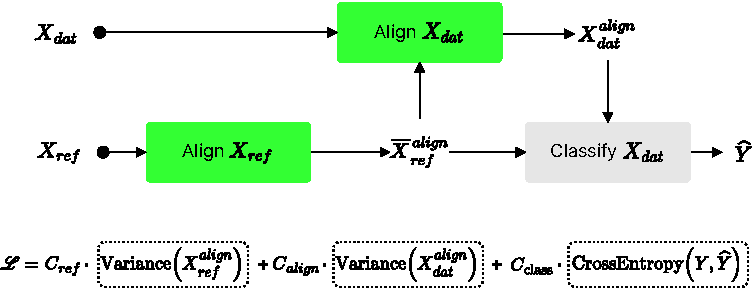
\includegraphics[width=\linewidth]{figures/phm4.pdf}}
    \caption{Overall strategy of the proposed classification model. It simultaneously 1) aligns reference data $X_{ref}$, 2) aligns pressure data $X_{dat}$ conditioned on the elastic average of the reference data and 3) classifies it to a given label $\hat{Y}$. 
    The final classification module is fed with aligned pressure data $X_{dat}$ and with the elastic average of reference data $X_{ref}$ as well.
    The loss function is defined as the weighted average of each task loss.}
    \label{fig:phm_method2}
    \end{center}
\end{figure}



\subsection{Alignment Module}
The alignment module is composed of a localization network, a CPA basis generator, ODE solver and a sampler. As mentioned in \cite{martinez2022closed}, the localization network is a neural network that takes the input data $X$ and produces a set of transformation parameters $\theta$. The CPA basis generator then creates a set of velocity coordinates $v$ that define a regular grid over the input data. Then, the ODE solver (which is also a differentiable module) integrates the velocity function and yields the diffeormorphic warping function $\phi$. Finally, the sampler uses the warping function $\boldsymbol{\phi}$ to sample the input data $X$ at the transformed coordinates.
The only add-inn of the reference alignment module is that this data is averaged after alignment.


\begin{figure}[!htb]
    \begin{center}
    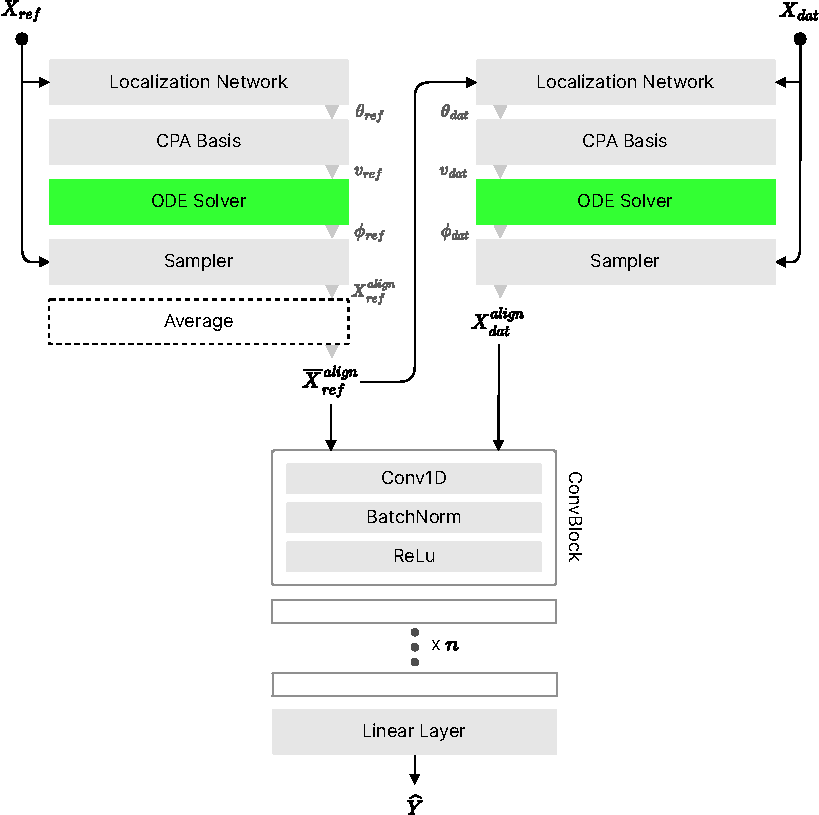
\includegraphics[width=\linewidth]{figures/phm3.pdf}
    \caption{Proposed model for time series classification. Reference data $X_{ref}$ is first aligned using the alignment module, which is composed of a localization network, a CPA basis generator, ODE solver and a sampler. An identical architecture is used to align pressure data $X_{dat}$. Note that in both cases, the localization network computes the alignment parameters $\theta_{ref}$ and $\theta_{dat}$ conditioned on the respective raw data $X_{ref}$ and $X_{dat}$. The classification module is composed of multiple convolutional blocks that estimate the fault class $\hat{Y}$ based on aligned data $X_{dat}^{align}$ and the elastic average of reference data $\bar{X}_{ref}^{align}$.}
    \label{fig:phm_method1}
    \end{center}
\end{figure}

\clearpage
\subsection{Classification Module}
The classification module consists of $n$ convolutional blocks and a fully-connected layer. The convolutional block is made of a 1D convolutional layer, a batch norm layer and a ReLU activation layer. 

In a \textbf{1D convolution}, a kernel or filter slides across the input signal, computing the dot product between the entries of the filter and the input, producing a new feature map. The goal of a 1D convolution is to extract local features and patterns from the input signal while reducing its length, preserving spatial information and relations between values (see \cref{fig:phm_convolution}). 1D convolutions can inherently capture some shift invariance in the data, but note that these are not shift-invariant but shift-equivariant: a shift of the input to a convolutional layer produces a shift in the output feature maps by the same amount. Therefore, these convolutional layers serve to additionally eliminate any remaining warping present in the aligned data.

% CONVOLUTION
\begin{figure}[!htb]
    \begin{center}
    % \scalebox{1.0}{
        \begin{tikzpicture}[arr/.style={matrix of nodes, nodes={draw}}]
            
            \matrix(A) [arr]
            {
              0 & 1 & 1 & |[fill=orange!30]| 2 & |[fill=orange!30]| 4 & |[fill=orange!30]| 0 & 1 & 1 & 2 \\
            };
            \node[right=0.5 em of A] {Input $I$};
            
            
            \matrix (B) [arr, below=0.5em of A, nodes={draw, fill=red!30}]
            {
              0 & 2 & 1 \\
            };
            \node[right=4 em of B] {Filter $F$};

            \matrix (B1) [arr, below=0.5em of B]
            {
              0 & 8 & 0 \\
            };
            \node[right=4 em of B1] {$I*F$};

            \matrix (C) [arr, below=0.5em of B1]
            {
              3 & 4 & 8 & |[fill=blue!80!black!30]| 8 & 1 & 3 & 4 \\
            };
            
            \node[right=1.5 em of C] {Output $O$};


            \draw[dashed, thick, orange] (A-1-4.south west) -- (B-1-1.north west);
            \draw[dashed, thick, orange] (A-1-6.south east) -- (B-1-3.north east);

            \draw[dashed, thick, red] (B-1-1.south west) -- (B1-1-1.north west);
            \draw[dashed, thick, red] (B-1-3.south east) -- (B1-1-3.north east);

            \draw[dashed, thick, blue] (B1-1-1.south west) -- (C-1-4.north west);
            \draw[dashed, thick, blue] (B1-1-3.south east) -- (C-1-4.north east);

            \node[] at (0, -0.6){$\times$};
            \node[] at (0, -1.65){$=$};
            \node[] at (0, -2.7){$\oplus$};
        \end{tikzpicture}
    % }
\caption{1D convolution operator slides the filter across the input and records element-wise products. Input size $L_{in}=9$, kernel size $k=3$, padding $p=0$, stride $s=1$.}
\label{fig:phm_convolution}
\end{center}
\end{figure}


The kernel size, padding and stride hyperparameters determine how the filter interacts with the input signal. Padding refers to adding zero-valued elements to the edges of the input signal, allowing the filter to operate on the border elements of the input without reducing its spatial size. Stride refers to the number of positions the filter moves in each step along the input. A larger stride value results in a down-sampled output, while a smaller stride value allows the filter to capture more local information.
The output dimension for a input vector of size $L_{in}$, padding $p$, stride $s$ and kernel size $k$ can be computed as $1+(L_{in}+2p-s(k-1)-1)/s$.


A \textbf{batch norm layer} normalizes the activations of neurons for each channel across a mini-batch of data, helps to stabilize the learning process, reduce the covariate shift, and increase the training speed. 

\textbf{ReLU} (Rectified Linear Unit) is defined as $\varphi(x) = \max(0, x)$, where $x$ is the input to the activation function. Other activation functions can be used, as visualized in \cref{fig:phm_activation}. Major benefits of ReLUs are sparsity and a reduced likelihood of vanishing gradient. The constant gradient of ReLUs results in faster learning, whereas the gradient of sigmoids becomes increasingly small as the absolute value of $x$ increases. In addition, sigmoids are more likely to generate some non-zero value resulting in dense representations.

% ACTIVATION FUNCTIONS
\begin{figure}[!htb]
   \begin{center}
       \scalebox{0.9}{
       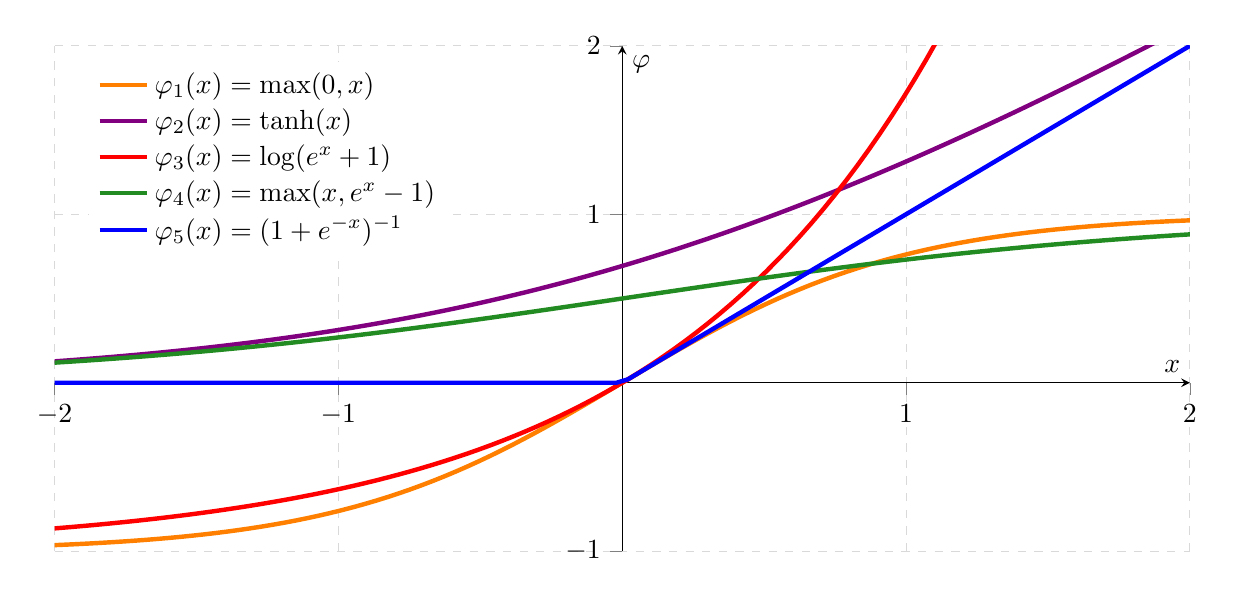
\begin{tikzpicture}
           \begin{axis}[
               legend pos=north west,
               legend cell align={left},
               legend style={draw=none},
               axis x line=middle,
               axis y line=middle,
               xtick={-2, -1, 1, 2},
               ytick={-1, 1, 2},
               grid = major,
               width=16cm,
               height=8cm,
               grid style={dashed, gray!30},
               xmin=-2,
               xmax= 2,
               ymin=-1,
               ymax= 2,
               %axis background/.style={fill=white},
               xlabel=$x$,
               ylabel=$\varphi$,
               tick align=outside,
               enlargelimits=false]
           % plot the stirling-formulae
           \addplot[domain=-2:2, orange, ultra thick,samples=100] {tanh(x)};
           \addplot[domain=-2:2, violet, ultra thick,samples=100] {ln(exp(x) + 1)};
           \addplot[domain=-2:2, red, ultra thick,samples=100] {max(x, exp(x) - 1)};
           \addplot[domain=-2:2, ForestGreen, ultra thick,samples=100] {1/(1+exp(-x))};
           \addplot[domain=-2:2, blue, ultra thick,samples=100] {max(0, x)};
           \addlegendentry{$\varphi_1(x)=\max(0, x)$}
           \addlegendentry{$\varphi_2(x)=\tanh(x)$}
           \addlegendentry{$\varphi_3(x)=\log(e^x + 1)$}
           \addlegendentry{$\varphi_4(x)=\max(x, e^x - 1)$}
           \addlegendentry{$\varphi_5(x)=(1+e^{-x})^{-1}$}
           \end{axis}
       \end{tikzpicture}
       }
\caption{Activation functions for neural networks.}
\label{fig:phm_activation}
\end{center}
\end{figure}

The final \textbf{linear layer} is a fully-connected neural network like the one shown in \cref{fig:phm_neural_network}.


% NN
\begin{figure}[!htb]
    \begin{center}
    \scalebox{1.0}{
    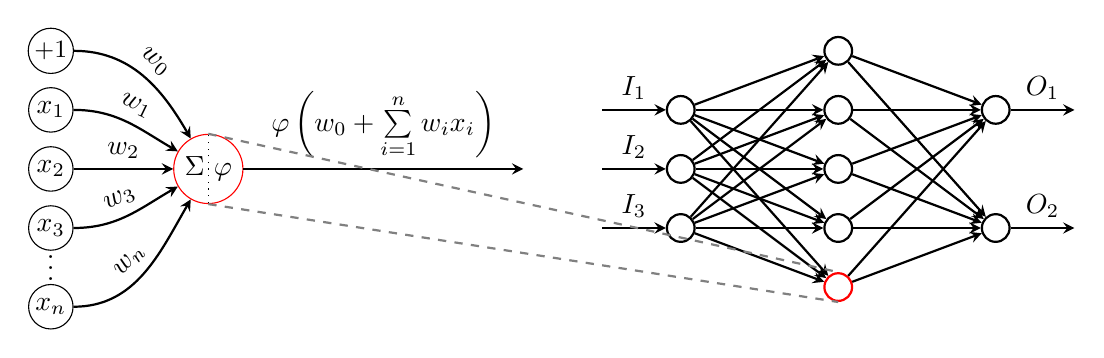
\begin{tikzpicture}
        \tikzstyle{inputNode}=[draw,circle,minimum size=10pt,inner sep=0pt]
        \tikzstyle{stateTransition}=[-stealth, thick]
    \node[draw,circle,red,minimum size=25pt,inner sep=0pt] (x) at (0,0) {\color{black}$\Sigma$ $\varphi$};

    \node[inputNode,text width=15pt,align=center] (x0) at (-2, 1.5) {\small $+1$};
    \node[inputNode,text width=15pt,align=center] (x1) at (-2, 0.75) {$x_1$};
    \node[inputNode,text width=15pt,align=center] (x2) at (-2, 0) {$x_2$};
    \node[inputNode,text width=15pt,align=center] (x3) at (-2, -0.75) {$x_3$};
    \node[inputNode,text width=15pt,align=center] (xn) at (-2, -1.75) {$x_n$};

    \draw[stateTransition] (x0) to[out=0,in=120] node [midway, sloped, above] {$w_0$} (x);
    \draw[stateTransition] (x1) to[out=0,in=150] node [midway, sloped, above] {$w_1$} (x);
    \draw[stateTransition] (x2) to[out=0,in=180] node [midway, sloped, above] {$w_2$} (x);
    \draw[stateTransition] (x3) to[out=0,in=210] node [midway, sloped, above] {$w_3$} (x);
    \draw[stateTransition] (xn) to[out=0,in=240] node [midway, sloped, above] {$w_n$} (x);
    \draw[stateTransition] (x) -- (4,0.) node [midway,above] {$\varphi\left(w_0 + \sum\limits_{i=1}^{n}{w_ix_i}\right)$};
    \draw[dotted] (0,-0.43) -- (0,0.43);
    \node (dots) at (-2, -1.15) {$\vdots$};
    \node[inputNode, thick] (i1) at (6, 0.75) {};
    \node[inputNode, thick] (i2) at (6, 0) {};
    \node[inputNode, thick] (i3) at (6, -0.75) {};

    \node[inputNode, thick] (h1) at (8, 1.5) {};
    \node[inputNode, thick] (h2) at (8, 0.75) {};
    \node[inputNode, thick] (h3) at (8, 0) {};
    \node[inputNode, thick] (h4) at (8, -0.75) {};
    \node[inputNode, thick, red] (h5) at (8, -1.5) {};

    \node[inputNode, thick] (o1) at (10, 0.75) {};
    \node[inputNode, thick] (o2) at (10, -0.75) {};

    \draw[stateTransition] (5, 0.75) -- node[above] {$I_1$} (i1);
    \draw[stateTransition] (5, 0) -- node[above] {$I_2$} (i2);
    \draw[stateTransition] (5, -0.75) -- node[above] {$I_3$} (i3);

    \draw[stateTransition] (i1) -- (h1);
    \draw[stateTransition] (i1) -- (h2);
    \draw[stateTransition] (i1) -- (h3);
    \draw[stateTransition] (i1) -- (h4);
    \draw[stateTransition] (i1) -- (h5);
    \draw[stateTransition] (i2) -- (h1);
    \draw[stateTransition] (i2) -- (h2);
    \draw[stateTransition] (i2) -- (h3);
    \draw[stateTransition] (i2) -- (h4);
    \draw[stateTransition] (i2) -- (h5);
    \draw[stateTransition] (i3) -- (h1);
    \draw[stateTransition] (i3) -- (h2);
    \draw[stateTransition] (i3) -- (h3);
    \draw[stateTransition] (i3) -- (h4);
    \draw[stateTransition] (i3) -- (h5);

    \draw[stateTransition] (h1) -- (o1);
    \draw[stateTransition] (h1) -- (o2);
    \draw[stateTransition] (h2) -- (o1);
    \draw[stateTransition] (h2) -- (o2);
    \draw[stateTransition] (h3) -- (o1);
    \draw[stateTransition] (h3) -- (o2);
    \draw[stateTransition] (h4) -- (o1);
    \draw[stateTransition] (h4) -- (o2);
    \draw[stateTransition] (h5) -- (o1);
    \draw[stateTransition] (h5) -- (o2);

    % \node[above=of i1, align=center] (l1) {Input \\ layer};
    % \node[right=2.3em of l1, align=center] (l2) {Hidden \\ layer};
    % \node[right=2.3em of l2, align=center] (l3) {Output \\ layer};

    \draw[stateTransition] (o1) -- node[above] {$O_1$} (11, 0.75);
    \draw[stateTransition] (o2) -- node[above] {$O_2$} (11, -0.75);

    \path[dashed, double, thick, gray] (x.north) edge[bend left=0] (h5.north);
    \path[dashed, double, thick, gray] (x.south) edge[bend right=0] (h5.south);
    \end{tikzpicture}
    }
    \caption{Illustration of a fully-connected neural network, also known as a linear layer.}
    \label{fig:phm_neural_network}
    \end{center}
\end{figure}


    




\clearpage
\section{Experiments and Results}\label{sec:results_4}



\subsection{Experimental Setup}

% \subsection{Dataset \& Prediction Task}

% \subsection{Baseline CNN Architecture}
% As a baseline with which to compare, we considered a CNN without any additional alignment. 
% \subsection{CNN Baseline vs Transformer Network}

The proposed classification model is trained with the training set made available by the organizers of the PHM Data Challenge.
Multivariate time series of pressure sensor readings $X_{dat}$, and their corresponding class $Y$ from a fleet of eight individuals are provided. A label of 1 represents the No-Fault condition, and a label of 2-11 corresponds to different fault types. 
The reference measurements $X_{ref}$ for each individual are included as well. 
The objective of the classification model is to predict the label $Y$ for each cycle.
% Five individuals are supplied as training, including their labels. One individual is used for online scoring with a limited number of evaluations per day. 
Evaluation of the model performance is carried out using the independent test and validation sets, using the accuracy metric:
\begin{equation}\label{eq:phm_accuracy}
\text{Accuracy} = \cfrac{\text{Correctly classified cycles}}{\text{Total number of cycles}}
\end{equation}
Regarding the data structure, a three-dimensional tensor is used (see \cref{fig:channel}), where each row contains one impact cycle, the column dimension represents time and the channel dimension corresponds to the three sensor locations (\textit{pin, po, pdin}). The length of the data varies between different cycles.



% ROW/COLUMN/CHANNEL
\begin{figure}[!htb]
\begin{center}
\scalebox{0.8}{
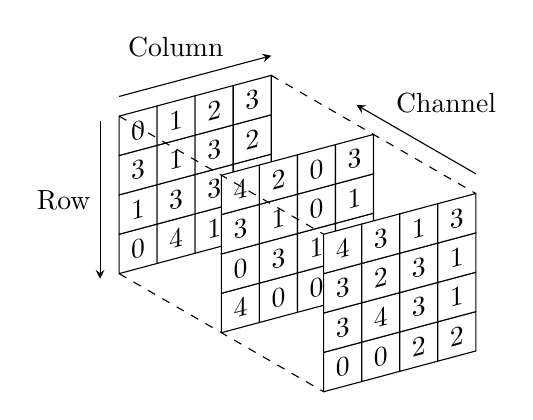
\begin{tikzpicture}[x=(15:.5cm), y=(90:.5cm), z=(330:.5cm), >=stealth]
	\draw [dashed] (0, 0, 0) -- (0, 0, 6) (4, 0, 0) -- (4, 0, 6);
	\foreach \z in {0, 3, 6} \foreach \x in {0,...,3}
	  \foreach \y [evaluate={\b=random(0, 4);}] in {0,...,3}
	    \filldraw [fill=white] (\x, \y, \z) -- (\x+1, \y, \z) -- (\x+1, \y+1, \z) --
	      (\x, \y+1, \z) -- cycle (\x+.5, \y+.5, \z) node [yslant=tan(15)] {\b};
	\draw [dashed] (0, 4, 0) -- (0, 4, 6) (4, 4, 0) -- (4, 4, 6);
	\draw [->] (0, 4.5, 0)  -- (4, 4.5, 0)   node [near end, above left] {Column};
	\draw [->] (-.5, 4, 0)  -- (-.5, 0, 0)   node [midway, left] {Row};
	\draw [->] (4, 4.5, 6) -- (4, 4.5, 2.5) node [near end, above right] {Channel};
\end{tikzpicture}
}
\vspace{-0.5cm}
\end{center}
\caption{Data is structured as a three-dimensional tensor.}
\label{fig:channel}
\end{figure}


Both localization networks are composed of 3 identical convolutional blocks, where each block contains a 1D convolutional layer followed by a BatchNorm and a ReLu activation layer. The 1D convolution operation has 10 filters, kernel size 8 and unit stride. The padding is chosen to match the output and input dimensions.
Regarding the CPA basis, the number of cells of the piecewise velocity function is set to 100 ($N_{\mathcal{P}}=100$) and the zero-boundary additional constraint is applied. The ODE solver uses 4 scaling-and-squaring iterations of the closed-form method presented in \cite{martinez2022closed}.

The classification module is composed of 3 identical convolutional blocks, where each block contains a 1D convolutional layer followed by a BatchNorm and a ReLu activation layer, as illustrated in \cref{fig:phm_method1}. The 1D convolution operation has 128 filters, kernel size 8 and unit stride. The padding is chosen to match the output and input dimensions. Aligned data $\bar{X}_{ref}^{align}$ and $X_{dat}^{align}$ are concatenated across the last dimension, so the classification module receives a three-dimensional tensor input with 6 channels (3 + 3), each corresponding to the three sensor locations (\textit{pin, po, pdin}). The output dimension is set to the number of classes (11).

The network was initialized with Xavier initialization \cite{glorot2010understanding} using a normal distribution and was trained for 100 epochs with $8e^{-5}$ learning rate, a batch size of $64$ and Adam \cite{kingma2014adam} optimizer with $\beta_{1}=0.9$, $\beta_{2}=0.999$ and $\epsilon=1e^{-8}$.

% \subsection{Implementation Details}
\subsection{Accuracy Results}
The hyperparameters of the loss function were optimized: $C_{ref}$ weights the variance of the aligned reference data $X_{ref}$, $C_{align}$ the variance of the raw data $X_{dat}$, and $C_{class}$ penalizes the classification cross-entropy. A grid-search was conducted from predefined sets of values: $C_{ref}=\{0,1,10,50,100\}$, $C_{align}=\{0,1,10,50,100\}$ and $C_{class}=\{1,10\}$.
\cref{tab:phm_hyperparameters} shows the train and test loss and accuracy values. Note how the baseline classification model without alignment ($C_{align}=0$, $C_{ref}=0$, $C_{class}=1$) scored significantly lower accuracy ($0.9715$) than the other cases where the alignment contributes in less or more measure ($C_{align}>0$ and $C_{ref}>0$). 
The grid-search analysis allowed to select the optimal weighting schemes, ensuring maximum accuracy. 
These experiments highlight the effectiveness of aligning time series data to reduce the risk of errors in classification by ensuring that the data is properly synchronized and accurately reflect the underlying patterns.



\small
\begingroup
\renewcommand\arraystretch{0.85}
\begin{longtable}{llr|rrrrrrrrrrrr}
    \caption{Grid-search analysis for the loss function hyperparameters}\label{tab:phm_hyperparameters}\\
    \toprule
    % $C_{\substack{align\\ref}}$ &  $C_{\substack{align\\dat}}$ &  $C_{class}$ &  $\mathcal{L}_{train}$ &  $\mathcal{L}_ {test}$ &  $\text{Accuracy}_{train}$ &  $\text{Accuracy}_{test}$ \\
    $C_{ref}$ &  $C_{align}$ &  $C_{class}$ &  $\mathcal{L}_{train}$ &  $\mathcal{L}_ {test}$ &  $\text{Accuracy}_{train}$ &  $\text{Accuracy}_{test}$ \\
    \midrule\endfirsthead
    \caption{(Cont.) Grid-search analysis for the loss function hyperparameters}\\
    \toprule
    $C_{ref}$ &  $C_{align}$ &  $C_{class}$ &  $\mathcal{L}_{train}$ &  $\mathcal{L}_{test}$ &  $\text{Accuracy}_{train}$ &  $\text{Accuracy}_{test}$ \\
    \midrule \endhead 
    % 0 &             0 &                   1 &     1.5692 &    1.5715 &     0.9940 &    0.9929 \\
    % 0 &             0 &                   1 &     1.8284 &    1.8393 &     0.7700 &    0.7676 \\
    % 0 &             0 &                   1 &     1.7877 &    1.7953 &     0.8326 &    0.8241 \\
    0 &             0 &                   1 &     1.6047 &    1.6072 &     0.9695 &    0.9715 \\
    1 &               1 &                    1 &      1.5433 &     1.5434 &     1.0000 &    1.0000 \\
    1 &              10 &                    1 &      1.5439 &     1.5440 &     1.0000 &    0.9999 \\
    1 &              50 &                    1 &      1.5510 &     1.5514 &     0.9997 &    0.9993 \\
    1 &             100 &                    1 &      1.5485 &     1.5486 &     1.0000 &    1.0000 \\
    10 &               1 &                    1 &      1.5432 &     1.5433 &     1.0000 &    1.0000 \\
    10 &              10 &                    1 &      1.5440 &     1.5440 &     1.0000 &    1.0000 \\
    10 &              50 &                    1 &      1.5523 &     1.5531 &     0.9995 &    0.9990 \\
    10 &             100 &                    1 &      1.5486 &     1.5489 &     1.0000 &    0.9999 \\
    50 &               1 &                    1 &      1.5464 &     1.5476 &     0.9996 &    0.9989 \\
    50 &              10 &                    1 &      1.5499 &     1.5517 &     0.9991 &    0.9975 \\
    50 &              50 &                    1 &      1.5509 &     1.5522 &     0.9999 &    0.9997 \\
    50 &             100 &                    1 &      1.5525 &     1.5532 &     1.0000 &    0.9996 \\
    100 &               1 &                    1 &      1.5432 &     1.5434 &     1.0000 &    0.9999 \\
    100 &              10 &                    1 &      1.5439 &     1.5440 &     1.0000 &    1.0000 \\
    100 &              50 &                    1 &      1.5513 &     1.5522 &     0.9997 &    0.9996 \\
    100 &             100 &                    1 &      1.5536 &     1.5542 &     0.9997 &    0.9999 \\
    1 &               1 &                   10 &     15.4643 &    15.4763 &     0.9998 &    0.9989 \\
    1 &              10 &                   10 &     15.4842 &    15.4912 &     0.9992 &    0.9989 \\
    1 &              50 &                   10 &     15.4825 &    15.4859 &     0.9978 &    0.9980 \\
    1 &             100 &                   10 &     15.4838 &    15.4921 &     0.9987 &    0.9988 \\
    10 &               1 &                   10 &     15.4618 &    15.4683 &     0.9992 &    0.9989 \\
    10 &              10 &                   10 &     15.5214 &    15.5309 &     0.9961 &    0.9964 \\
    10 &              50 &                   10 &     15.4708 &    15.4798 &     0.9996 &    0.9990 \\
    10 &             100 &                   10 &     15.4588 &    15.4696 &     0.9998 &    0.9990 \\
    50 &               1 &                   10 &     15.4554 &    15.4659 &     0.9994 &    0.9984 \\
    50 &              10 &                   10 &     15.4611 &    15.4665 &     0.9999 &    0.9997 \\
    50 &              50 &                   10 &     15.4883 &    15.5000 &     0.9996 &    0.9986 \\
    50 &             100 &                   10 &     15.4850 &    15.4956 &     0.9998 &    0.9994 \\
    100 &               1 &                   10 &     15.4645 &    15.4740 &     0.9995 &    0.9989 \\
    100 &              10 &                   10 &     15.4529 &    15.4656 &     0.9999 &    0.9990 \\
    100 &              50 &                   10 &     15.4674 &    15.4814 &     0.9992 &    0.9982 \\
    100 &             100 &                   10 &     15.5046 &    15.5177 &     0.9994 &    0.9985 \\
\bottomrule
\end{longtable}
\endgroup
\normalsize


\begin{figure}[!htb]
    \begin{center}
    \centerline{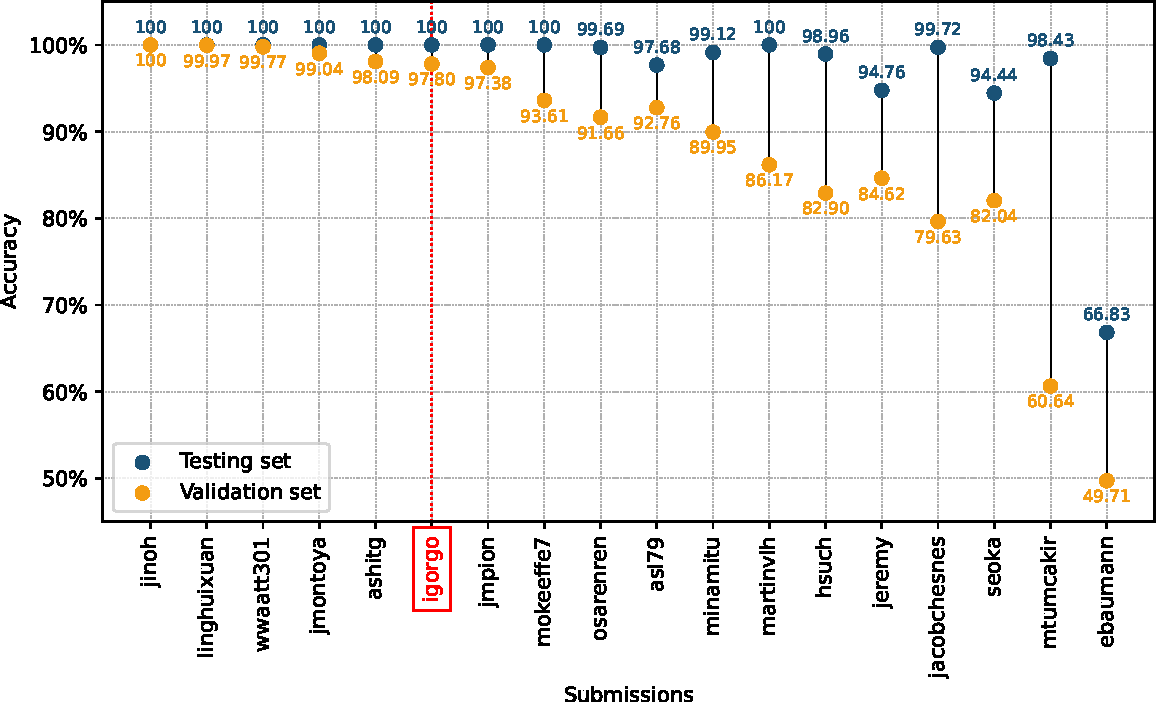
\includegraphics[width=\linewidth]{figures/challenge_results-crop.pdf}}
    \caption{Competition results in terms of accuracy. Test and validation sets. Extracted from \url{https://data.phmsociety.org/2022-phm-conference-data-challenge/}}
    \label{fig:phm_results}
    \end{center}
    % \vspace{-2cm}
\end{figure}


In the competition, the proposed model ranked sixth out of 18 competitors, with an accuracy of $100\%$ and $97.80\%$ for the test and validation sets respectively (see \cref{fig:phm_results}, our submission was named \textit{igorgo}). Overall, the model has shown high accuracy in classifying faulty signals and has demonstrated its robustness to variability and complexity in real-world time series data.


\subsection{Within-class Variance Reduction}

This section explores the reduction of within-class variance after alignment. This statistic provides an idea of how much temporal misalignment has been repaired. Results for all  (individual, channel) tuples are reported in \cref{fig:phm_variance}. 
The distribution of variance reduction varies depending on the channel and the extent of temporal misalignment. It is important to note that the decrease achieved in the train set is carried over to the test and validation sets, indicating that the model has been able to learn and generalize the warping misalignment in the data to unseen samples.

% \begin{table}[!htb]
%     \small
%     \caption{Reduction of variance per individual and channel (test \& validation sets).}
%     \label{tab:phm_variance}
%     \vspace{-0.5cm}
%     \begin{center}
%     \begin{tabular}{llll}
%         \toprule
%         Channel      &    pin &    pdin &      po \\
%         \midrule
%         Individual 1 &   5.9\% &  46.6\% &  25.4\% \\
%         Individual 2 &  10.1\% &  47.0\% &  28.1\% \\
%         Individual 3 &   8.9\% &  50.3\% &  26.5\% \\
%         Individual 4 &   4.1\% &  52.0\% &  27.1\% \\
%         Individual 5 &   5.5\% &  48.6\% &  25.3\% \\
%         Individual 6 &   6.2\% &  50.3\% &  24.9\% \\
%         Individual 7 &   1.7\% &  51.6\% &  27.8\% \\
%         Individual 8 &   6.4\% &  48.9\% &  28.0\% \\
%         \midrule
%         Overall Avg. &   6.1\% &  49.4\% &  26.6\% \\
%         \bottomrule
%     \end{tabular}
%     \end{center}
% \end{table}
% \vspace{-0.8cm}
\begin{figure}[!htb]
    \begin{center}
    \centerline{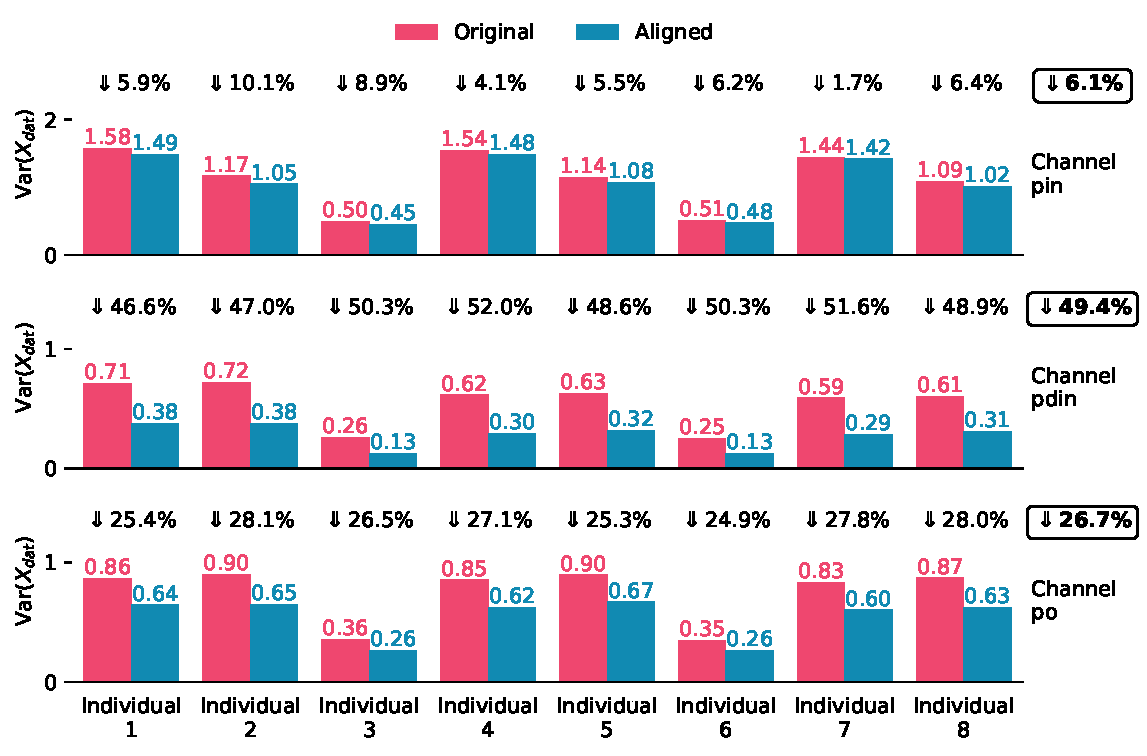
\includegraphics[width=\linewidth]{figures/results_variance_ext.pdf}}
    \vspace{-0.3cm}
    \caption{Reduction of variance per individual and channel (test \& validation sets).}
    \label{fig:phm_variance}
    \end{center}
    \vspace{-1cm}
\end{figure}


\subsection{Qualitative Alignment Results}

This section illustrates the visual differences before and after time series alignment. \cref{fig:phm_alignment_1a} represents the original training data before alignment, while \cref{fig:phm_alignment_1b} displays the aligned data from the test set.
The model learns to generalize alignments from the training set, so it does not need to solve a new optimization problem every time. The top graphic consists of a timeline of every time series instance (lines in \textcolor{gray}{gray}), and the Euclidean average (line in white) with one standard deviation shadow area (colored in translucent \textcolor{red}{red}). The heatmap on the bottom represents the time in the x-axis, each time series instance in the y-axis, and the color z-scale corresponds to the series value. This plot makes it easy to compare each time series, which may be overlapping at the top plot. Note the variance reduction between the left and right side. Results on more individuals were included in \cref{fig:phm_alignment_2}.

% \begin{figure}[!htb]
%     \begin{center}
%         \centerline{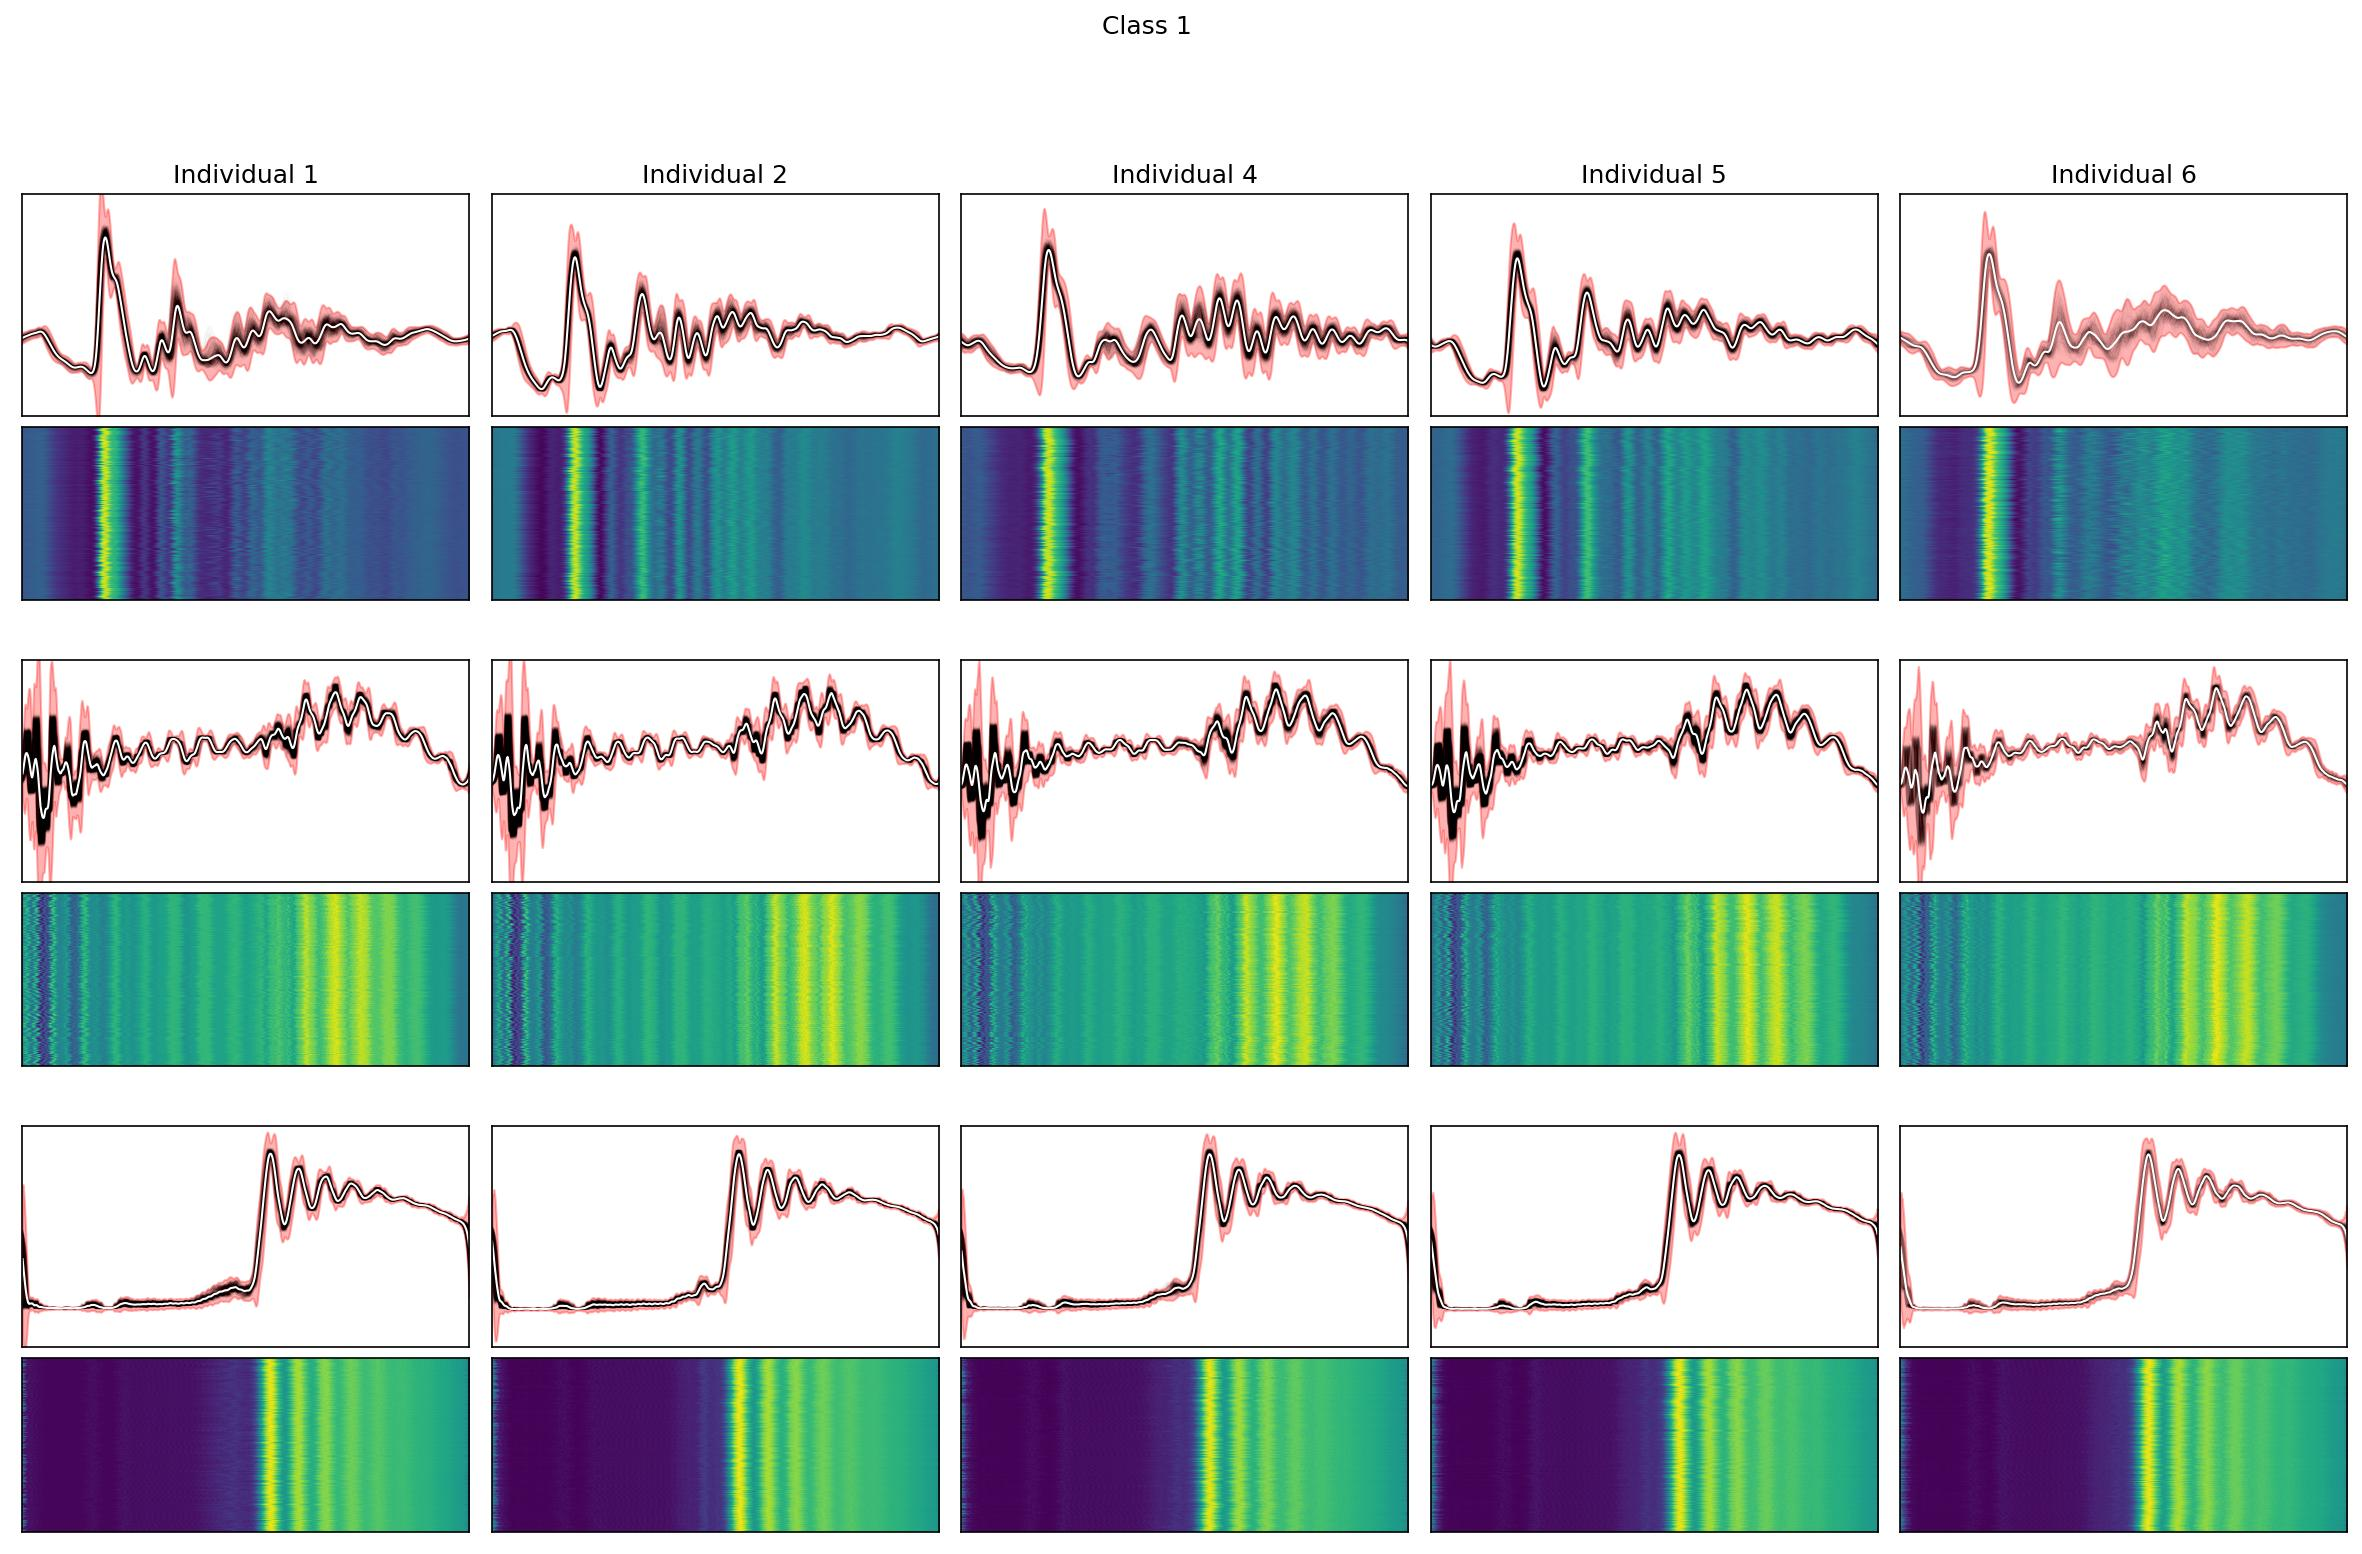
\includegraphics[width=\linewidth]{figures/original/plot_heatmap_class_1.jpg}}
%         \centerline{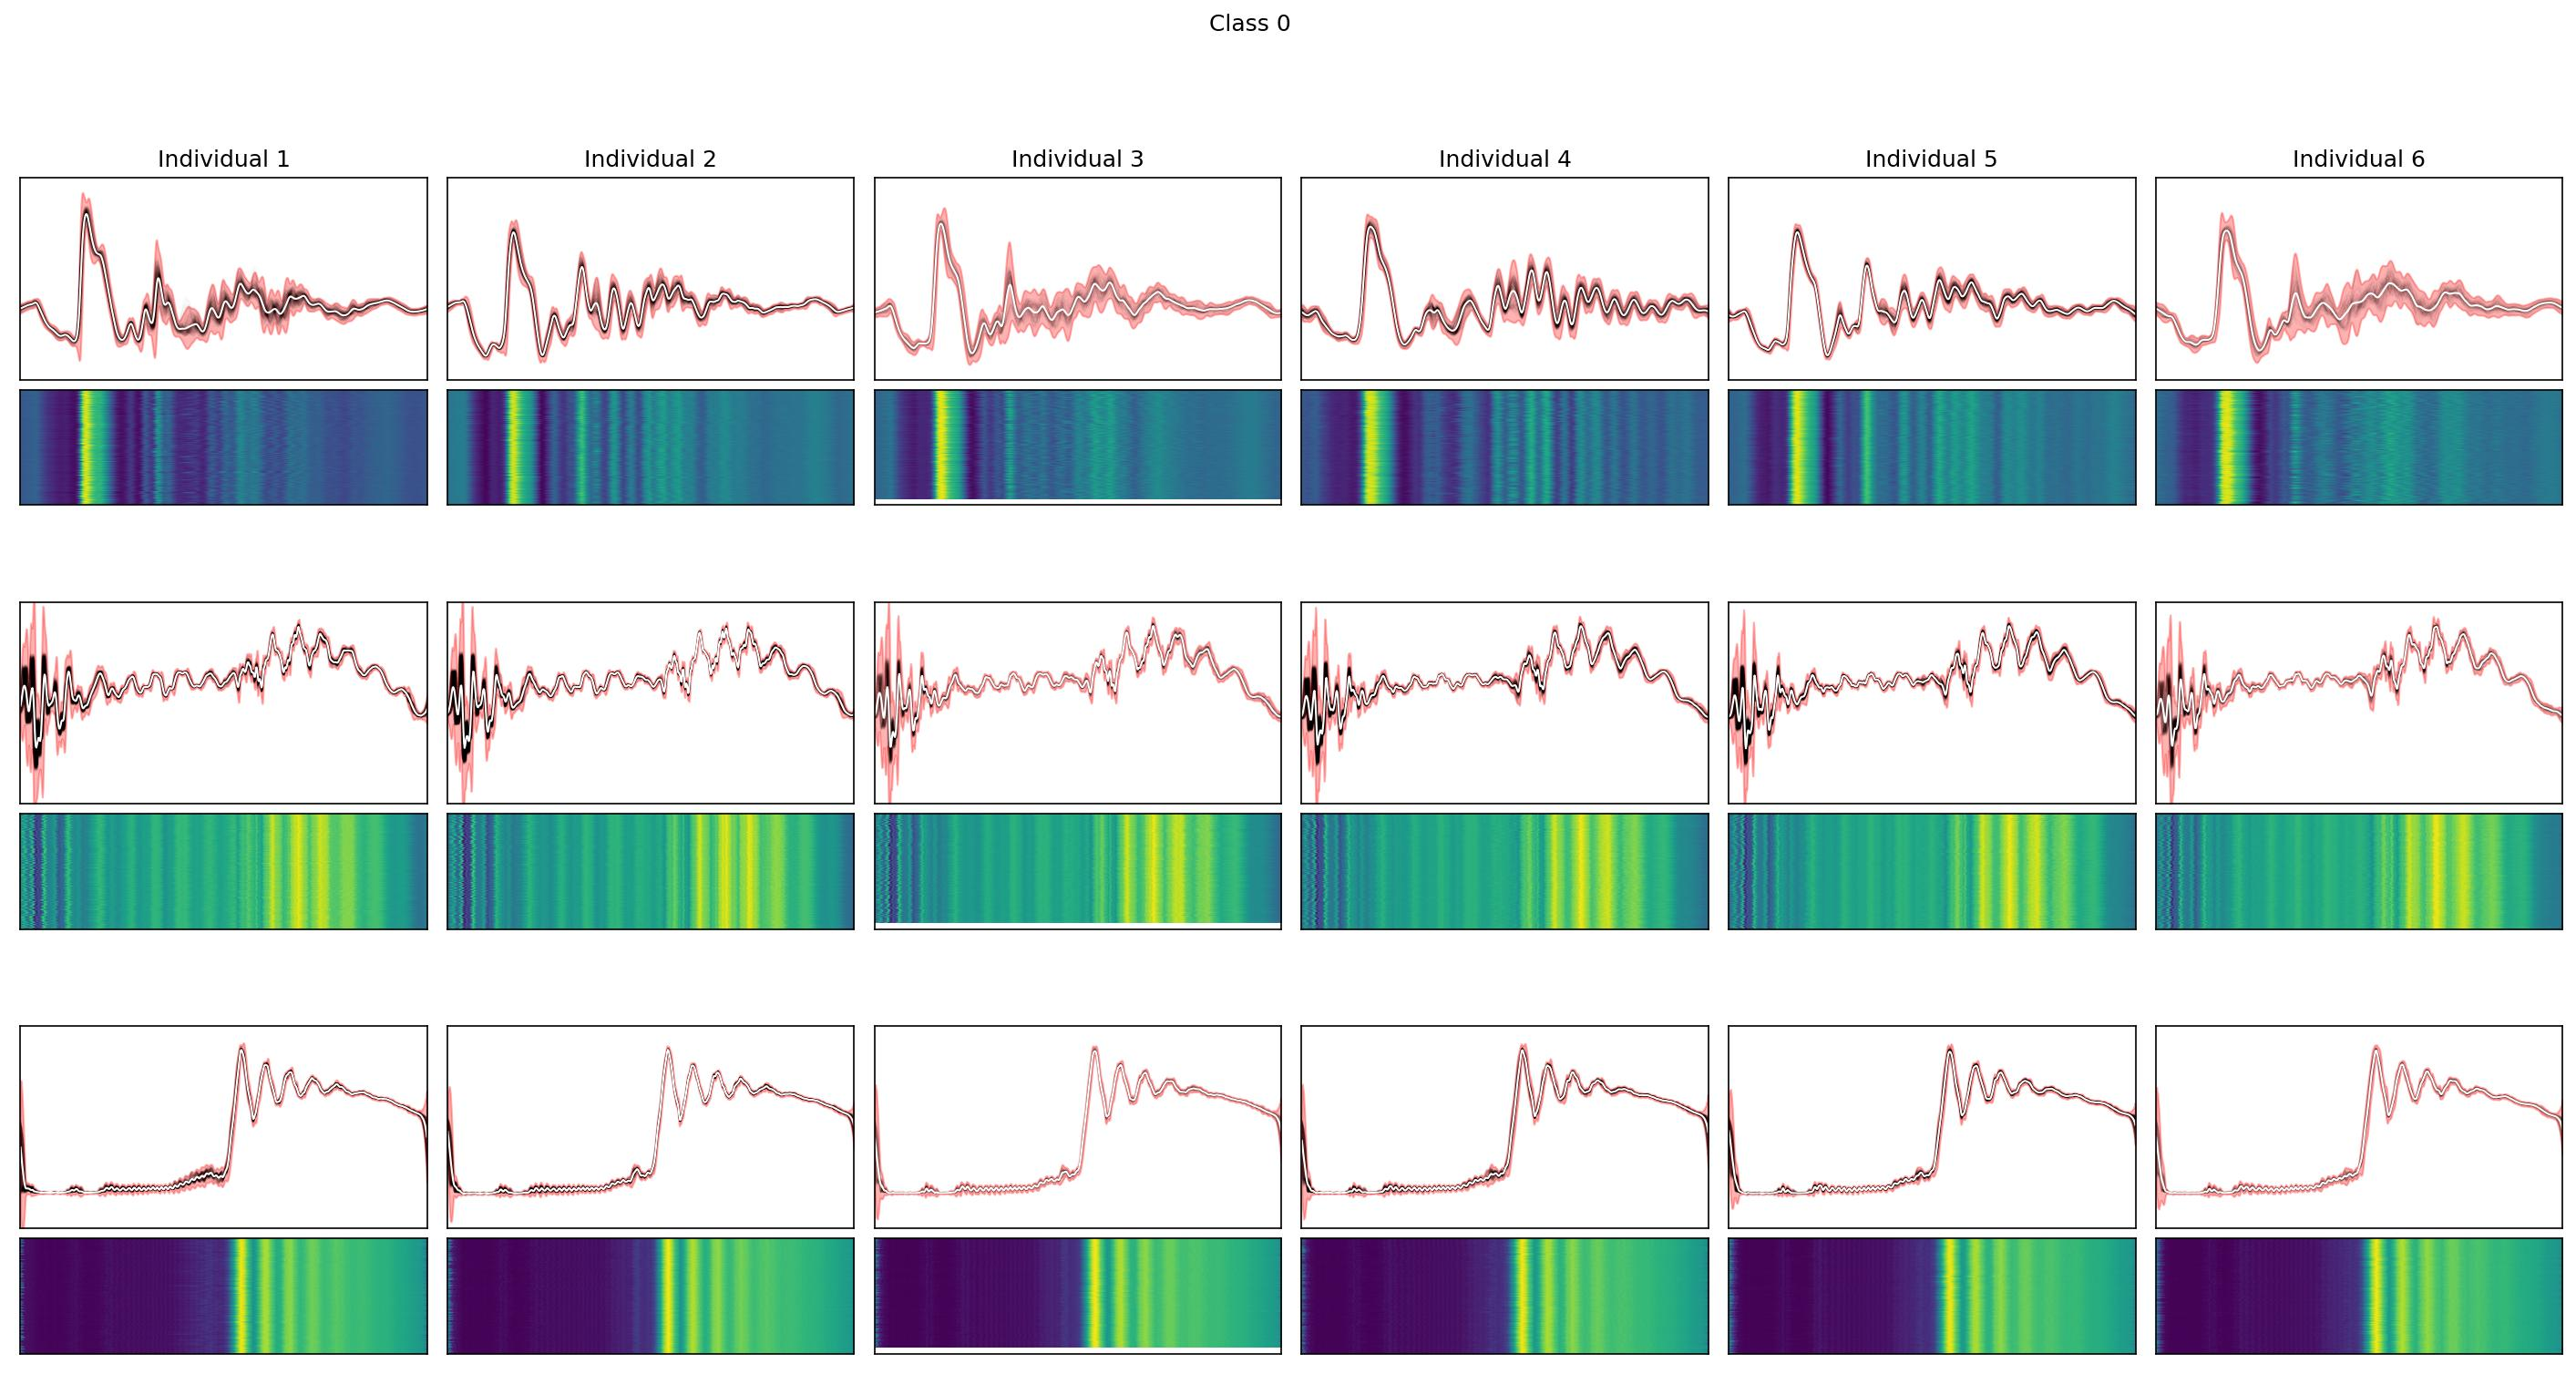
\includegraphics[width=\linewidth]{figures/aligned/plot_heatmap_class_1.jpg}}
%         \caption{}
%     \label{fig:phm_}
%     \end{center}
% \end{figure}

\begin{figure}[!htb]
    \begin{center}
        \begin{subfigure}[t]{\linewidth}
            \centering
            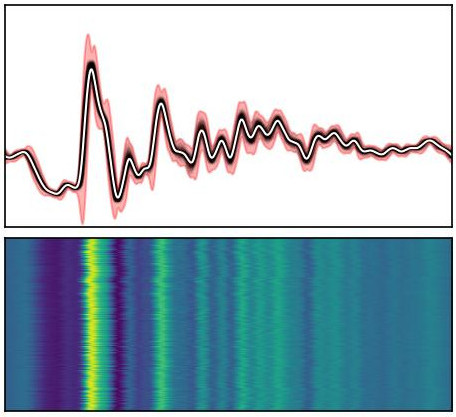
\includegraphics[width=0.32\linewidth]{figures/original/plot_heatmap_class_1_detail_1.jpg}
            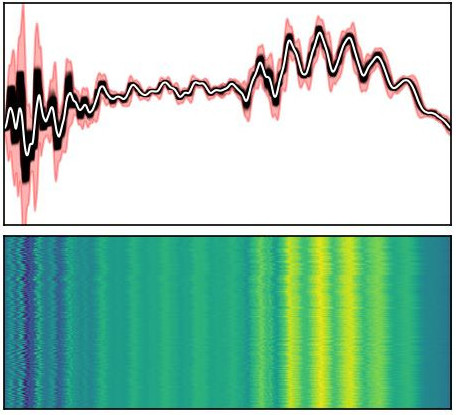
\includegraphics[width=0.32\linewidth]{figures/original/plot_heatmap_class_1_detail_2.jpg}
            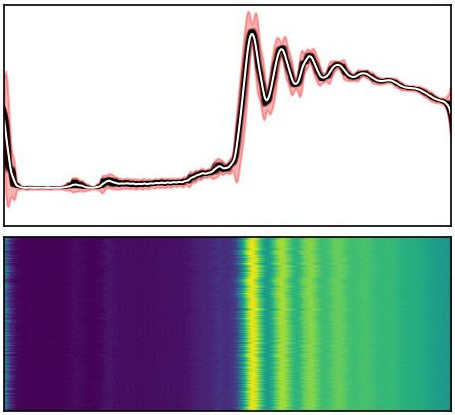
\includegraphics[width=0.32\linewidth]{figures/original/plot_heatmap_class_1_detail_3.jpg}
            \caption{Original data (training set)}
            \label{fig:phm_alignment_1a}
        \end{subfigure}
        % \hfill
        \begin{subfigure}[t]{\linewidth}
            \centering
            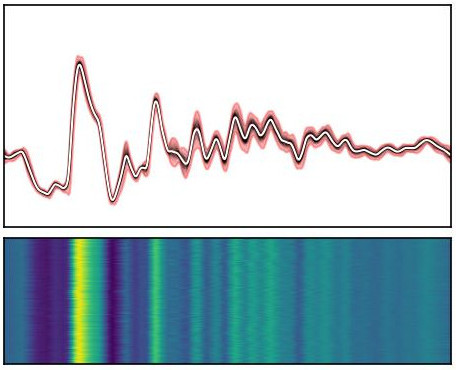
\includegraphics[width=0.32\linewidth]{figures/aligned/plot_heatmap_class_1_detail_1.jpg}
            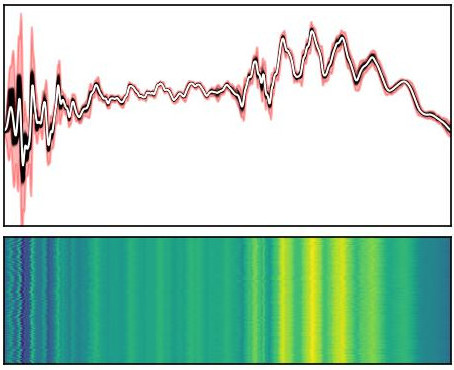
\includegraphics[width=0.32\linewidth]{figures/aligned/plot_heatmap_class_1_detail_2.jpg}
            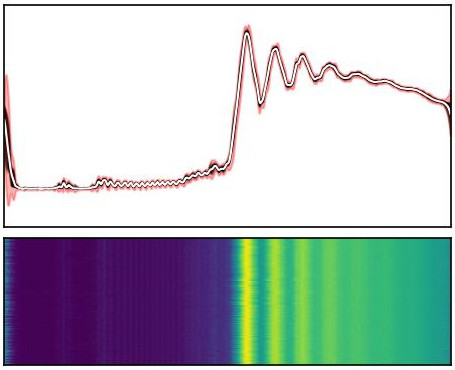
\includegraphics[width=0.32\linewidth]{figures/aligned/plot_heatmap_class_1_detail_3.jpg}
            \caption{Aligned data (test set)}
            \label{fig:phm_alignment_1b}
        \end{subfigure}
        \caption{Pressure sensor data before and after alignment: detail of one individual (number 5), and 3 channels (left: \textit{pin}, center: \textit{pdin}, right: \textit{po}). Note the reduction in the standard deviation after alignment, represented by the shadow area in translucent red color.}
    \label{fig:phm_alignment_1}
    \end{center}
\end{figure}

\begin{figure}[!htb]
    \begin{center}
    \begin{subfigure}{\linewidth}
        
\includegraphics[width=\linewidth]{figures/original/plot_heatmap_class_1_1.jpg}
        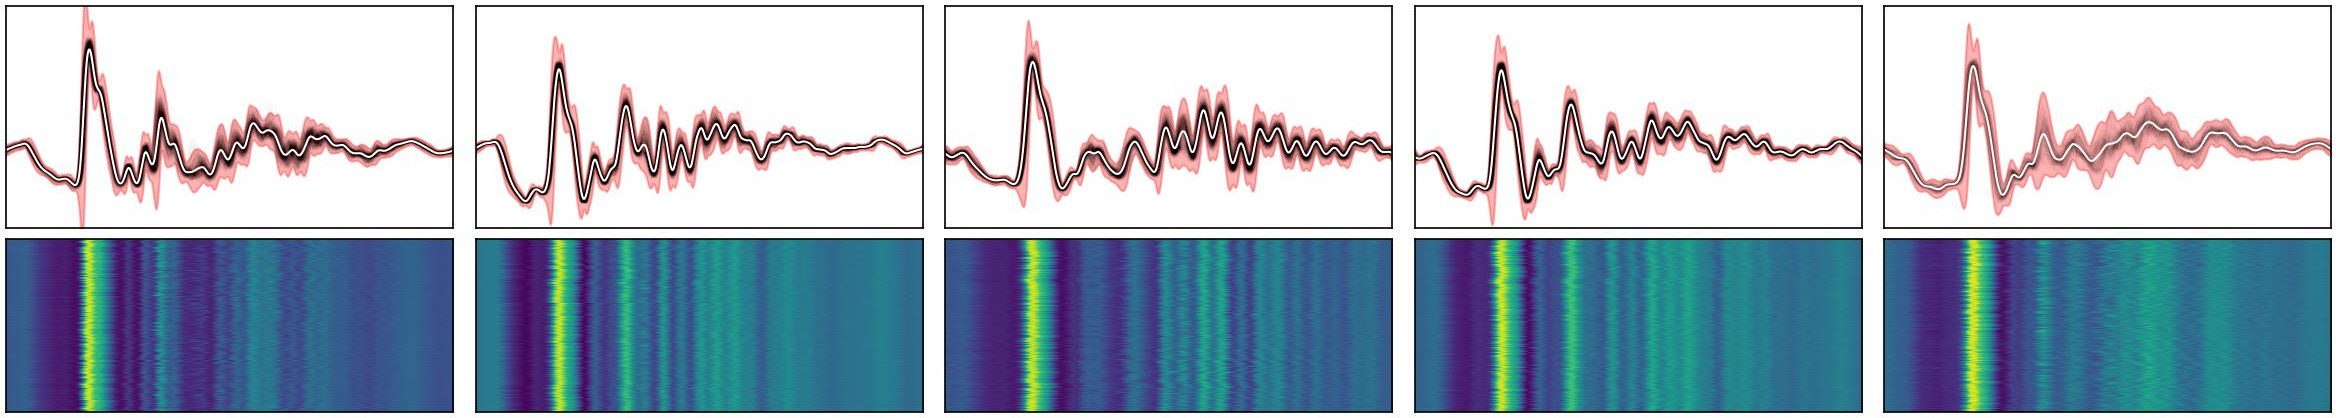
\includegraphics[width=\linewidth]{figures/original/plot_heatmap_class_1_2.jpg}
        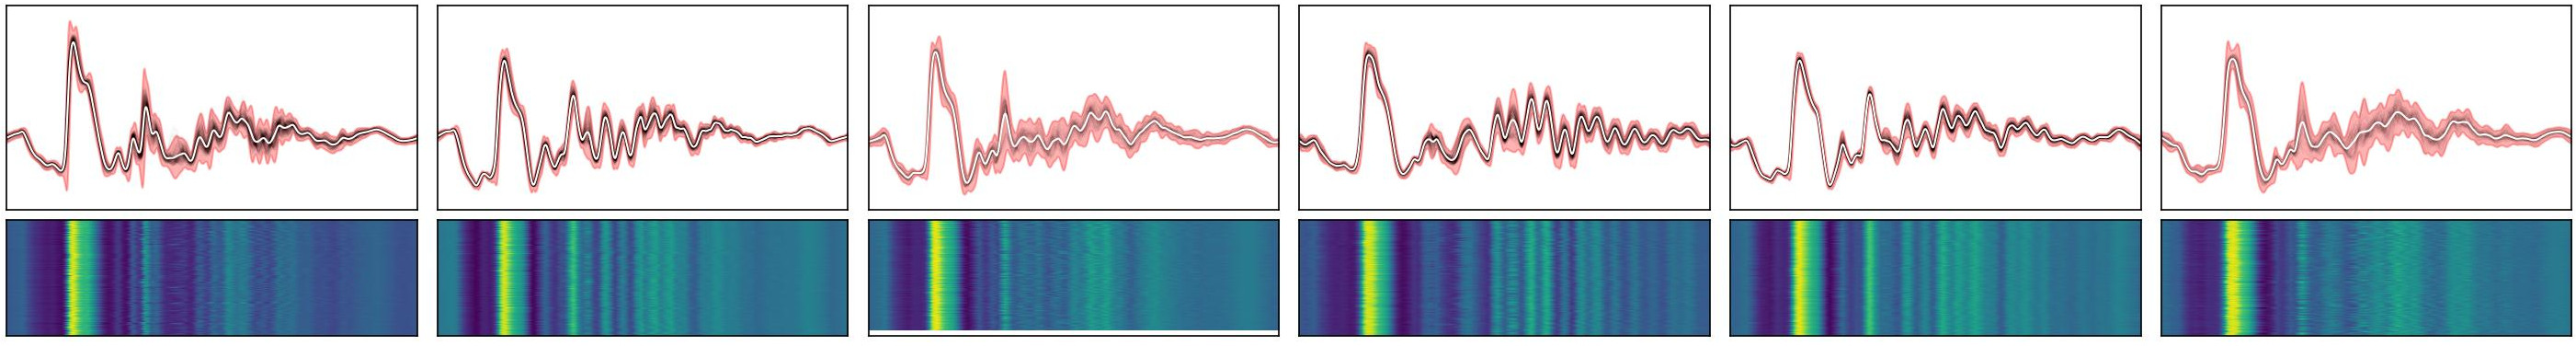
\includegraphics[height=0.161\linewidth,trim=0 0 900 0,clip]{figures/aligned/plot_heatmap_class_1_2.jpg}
        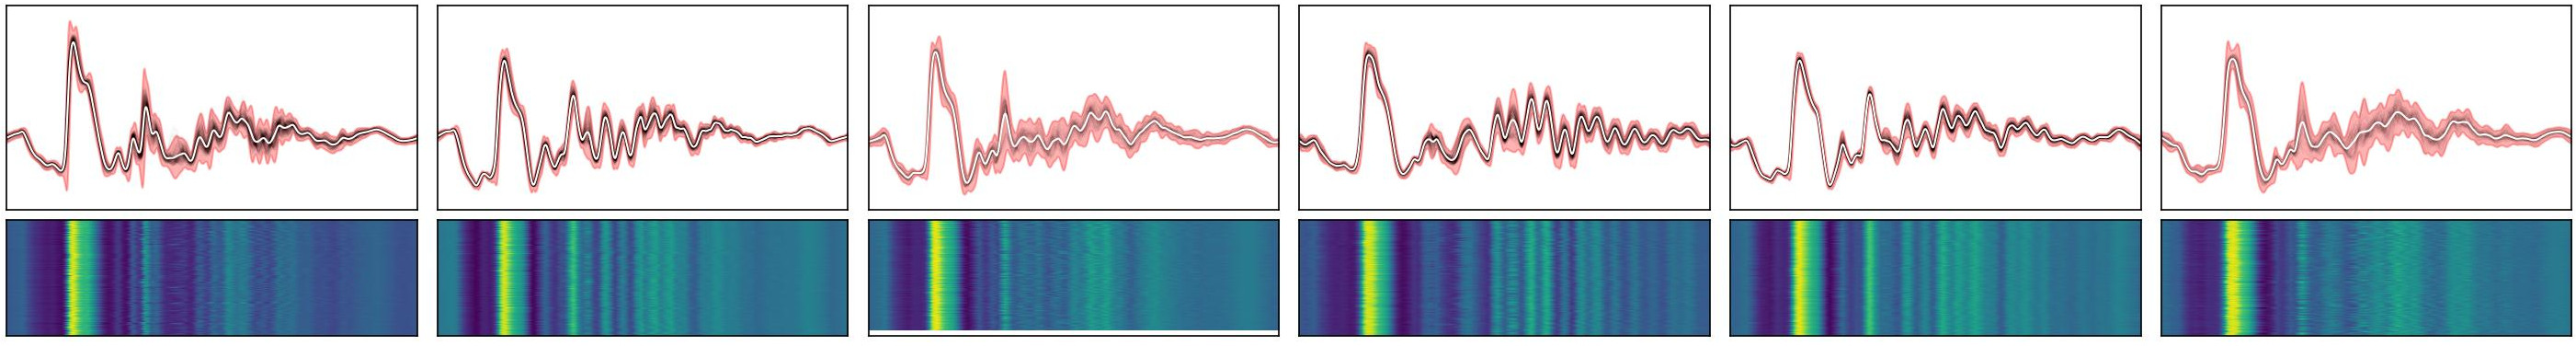
\includegraphics[height=0.161\linewidth,trim=675 0 0 0,clip]{figures/aligned/plot_heatmap_class_1_2.jpg}
        \caption{\textit{pin} sensor, with original data (training set) on top, and aligned data (test set) on the bottom.}
    \end{subfigure}
    \begin{subfigure}{\linewidth}
        
\includegraphics[width=\linewidth]{figures/original/plot_heatmap_class_1_1.jpg}
        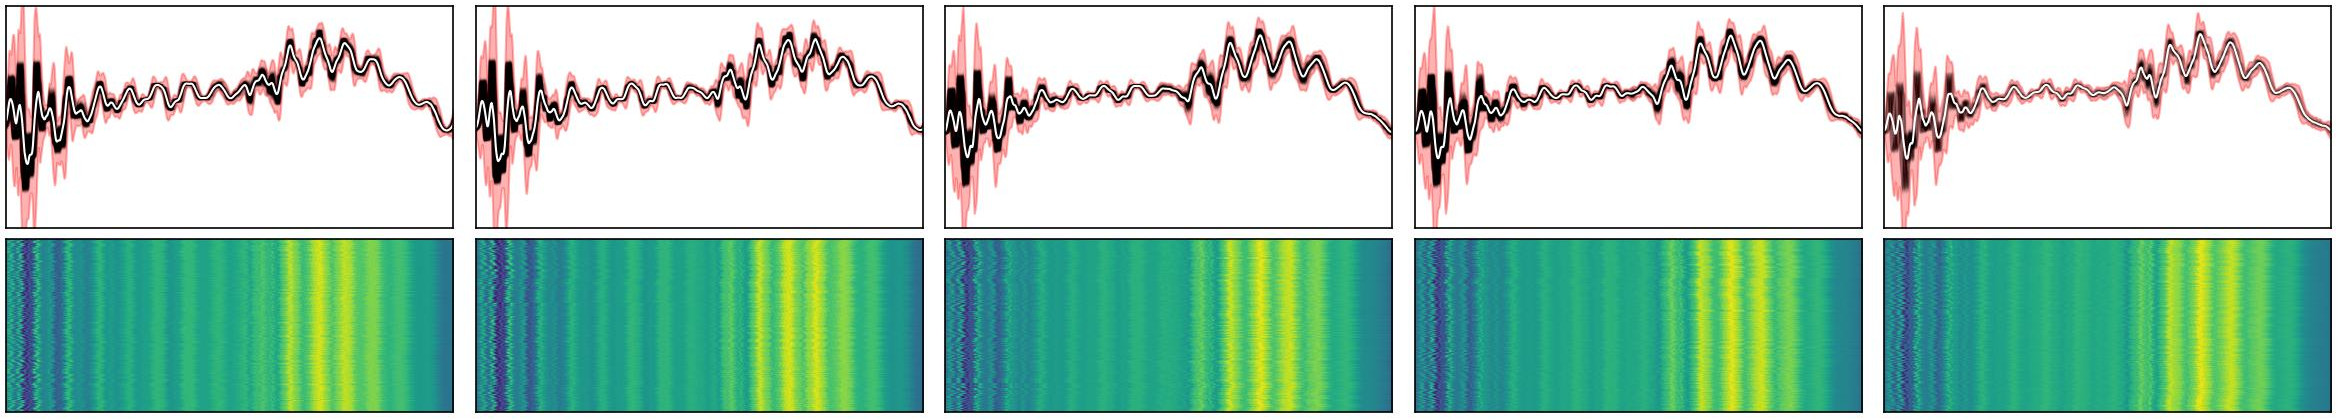
\includegraphics[width=\linewidth]{figures/original/plot_heatmap_class_1_3.jpg}
        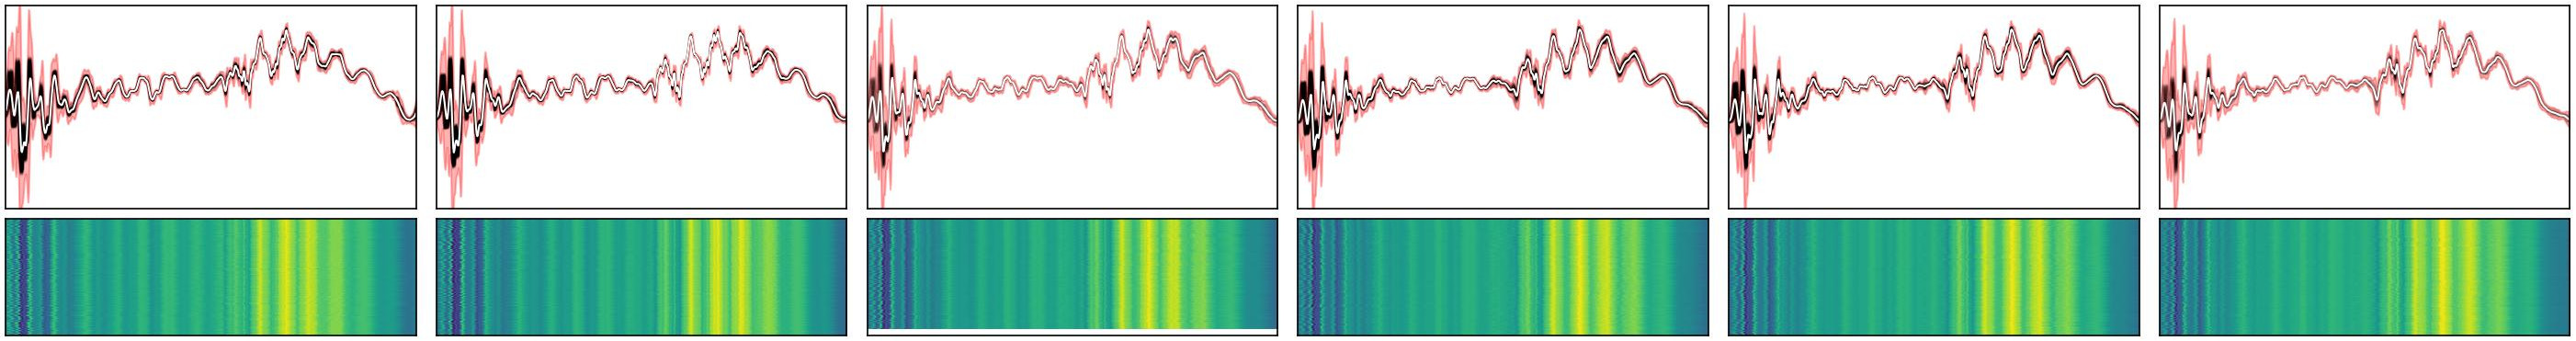
\includegraphics[height=0.159\linewidth,trim=0 0 900 0,clip]{figures/aligned/plot_heatmap_class_1_3.jpg}
        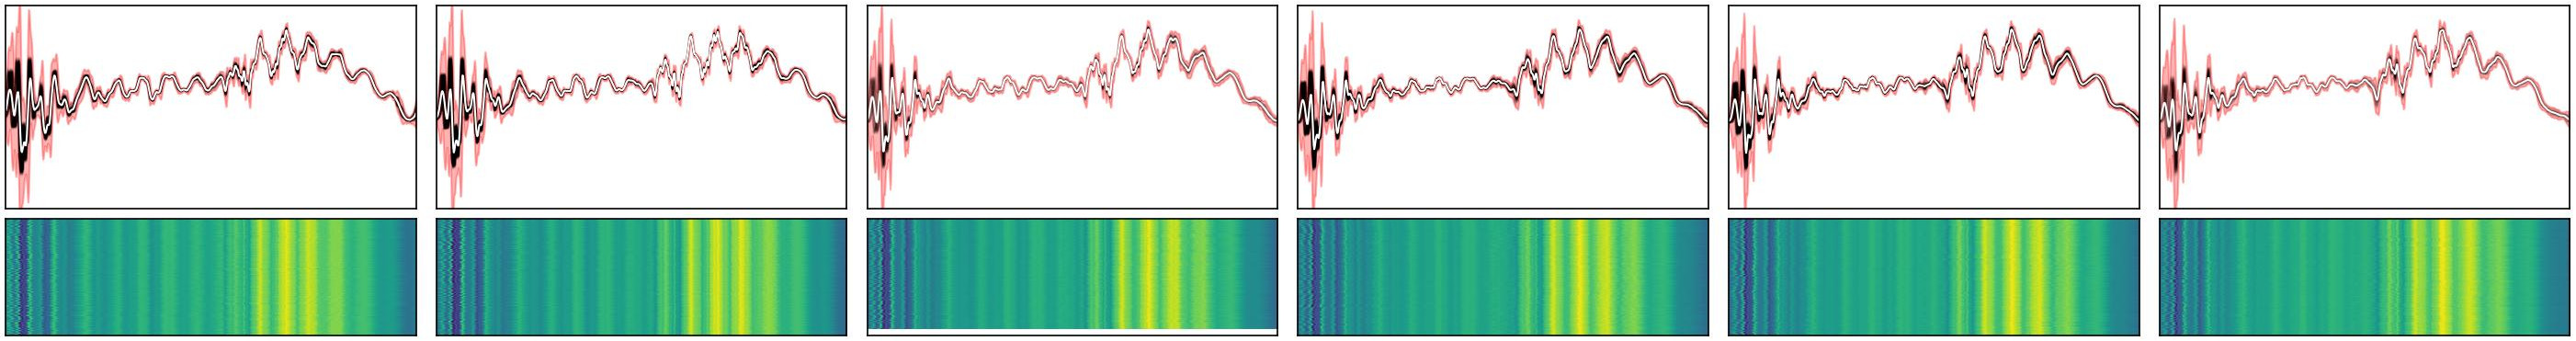
\includegraphics[height=0.159\linewidth,trim=675 0 0 0,clip]{figures/aligned/plot_heatmap_class_1_3.jpg}
        \caption{\textit{pdin} sensor, with original data (training set) on top, and aligned data (test set) on the bottom.}
    \end{subfigure}
    \begin{subfigure}{\linewidth}
        
\includegraphics[width=\linewidth]{figures/original/plot_heatmap_class_1_1.jpg}
        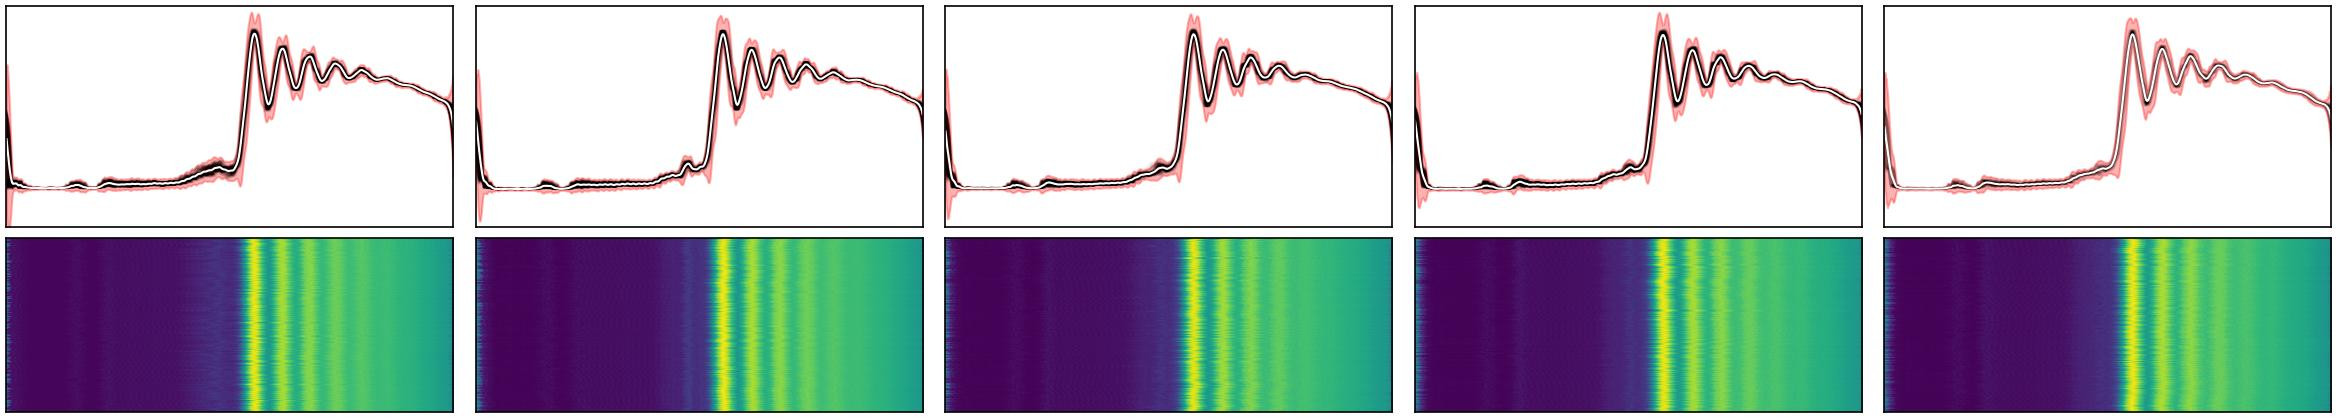
\includegraphics[width=\linewidth]{figures/original/plot_heatmap_class_1_4.jpg}
        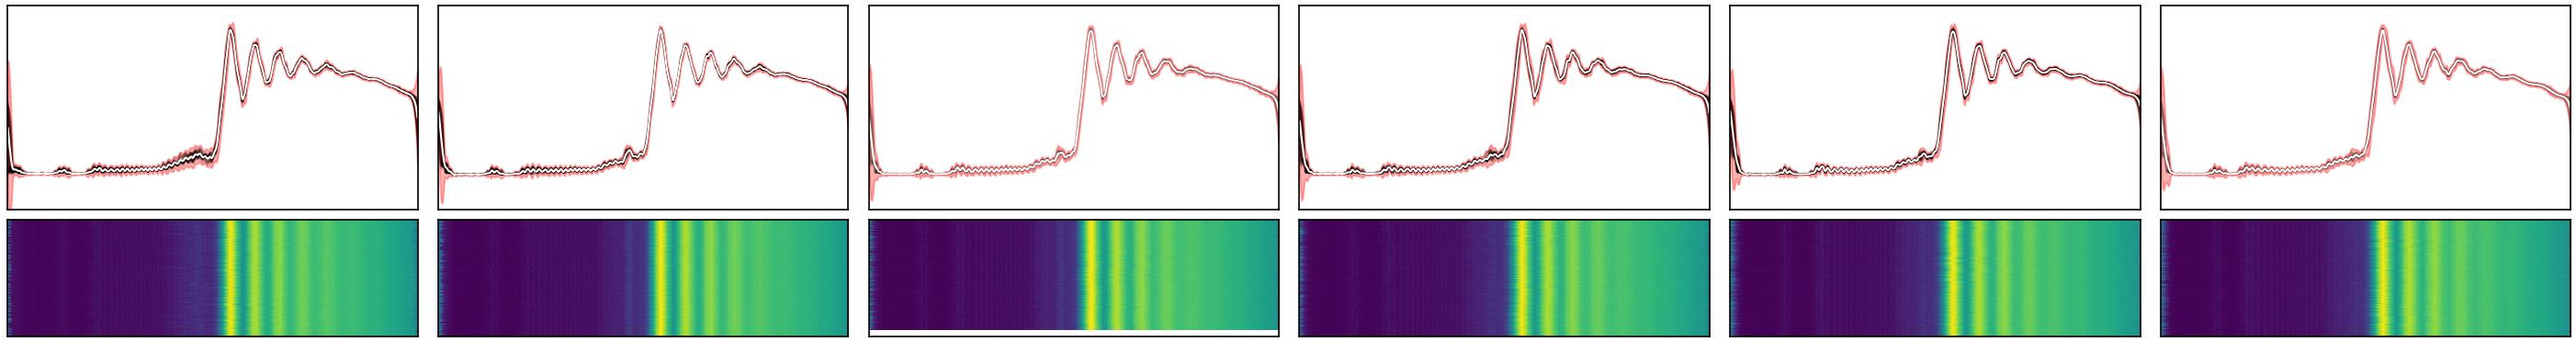
\includegraphics[height=0.159\linewidth,trim=0 0 900 0,clip]{figures/aligned/plot_heatmap_class_1_4.jpg}
        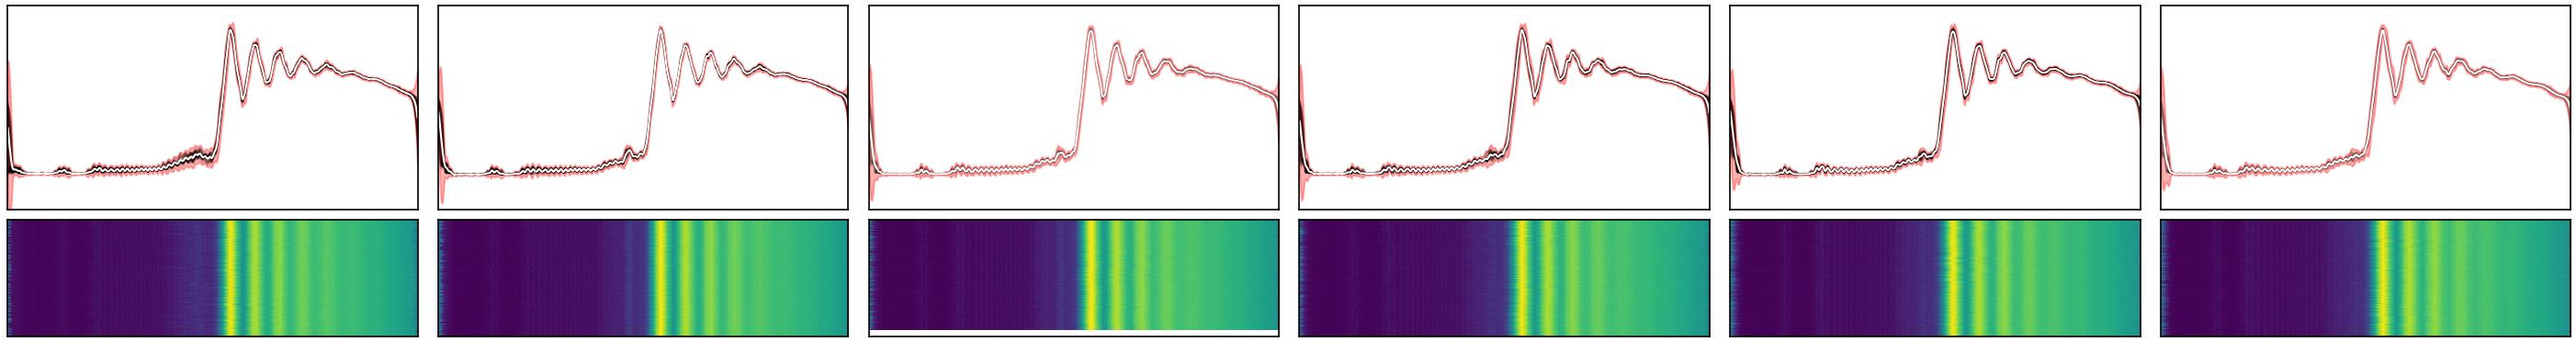
\includegraphics[height=0.159\linewidth,trim=675 0 0 0,clip]{figures/aligned/plot_heatmap_class_1_4.jpg}
        \caption{\textit{po} sensor, with original data (training set) on top, and aligned data (test set) on the bottom.}
    \end{subfigure}
    \caption{Pressure sensor data before and after alignment: multiple individuals (1,2,4,5,6), and 3 channels (top: \textit{pin}, middle: \textit{pdin}, bottom: \textit{po})}
    \label{fig:phm_alignment_2}
    \end{center}
\end{figure}

% \begin{figure}[!htb]
%     \begin{center}
%     \begin{subfigure}{\linewidth}
%         \centering
%         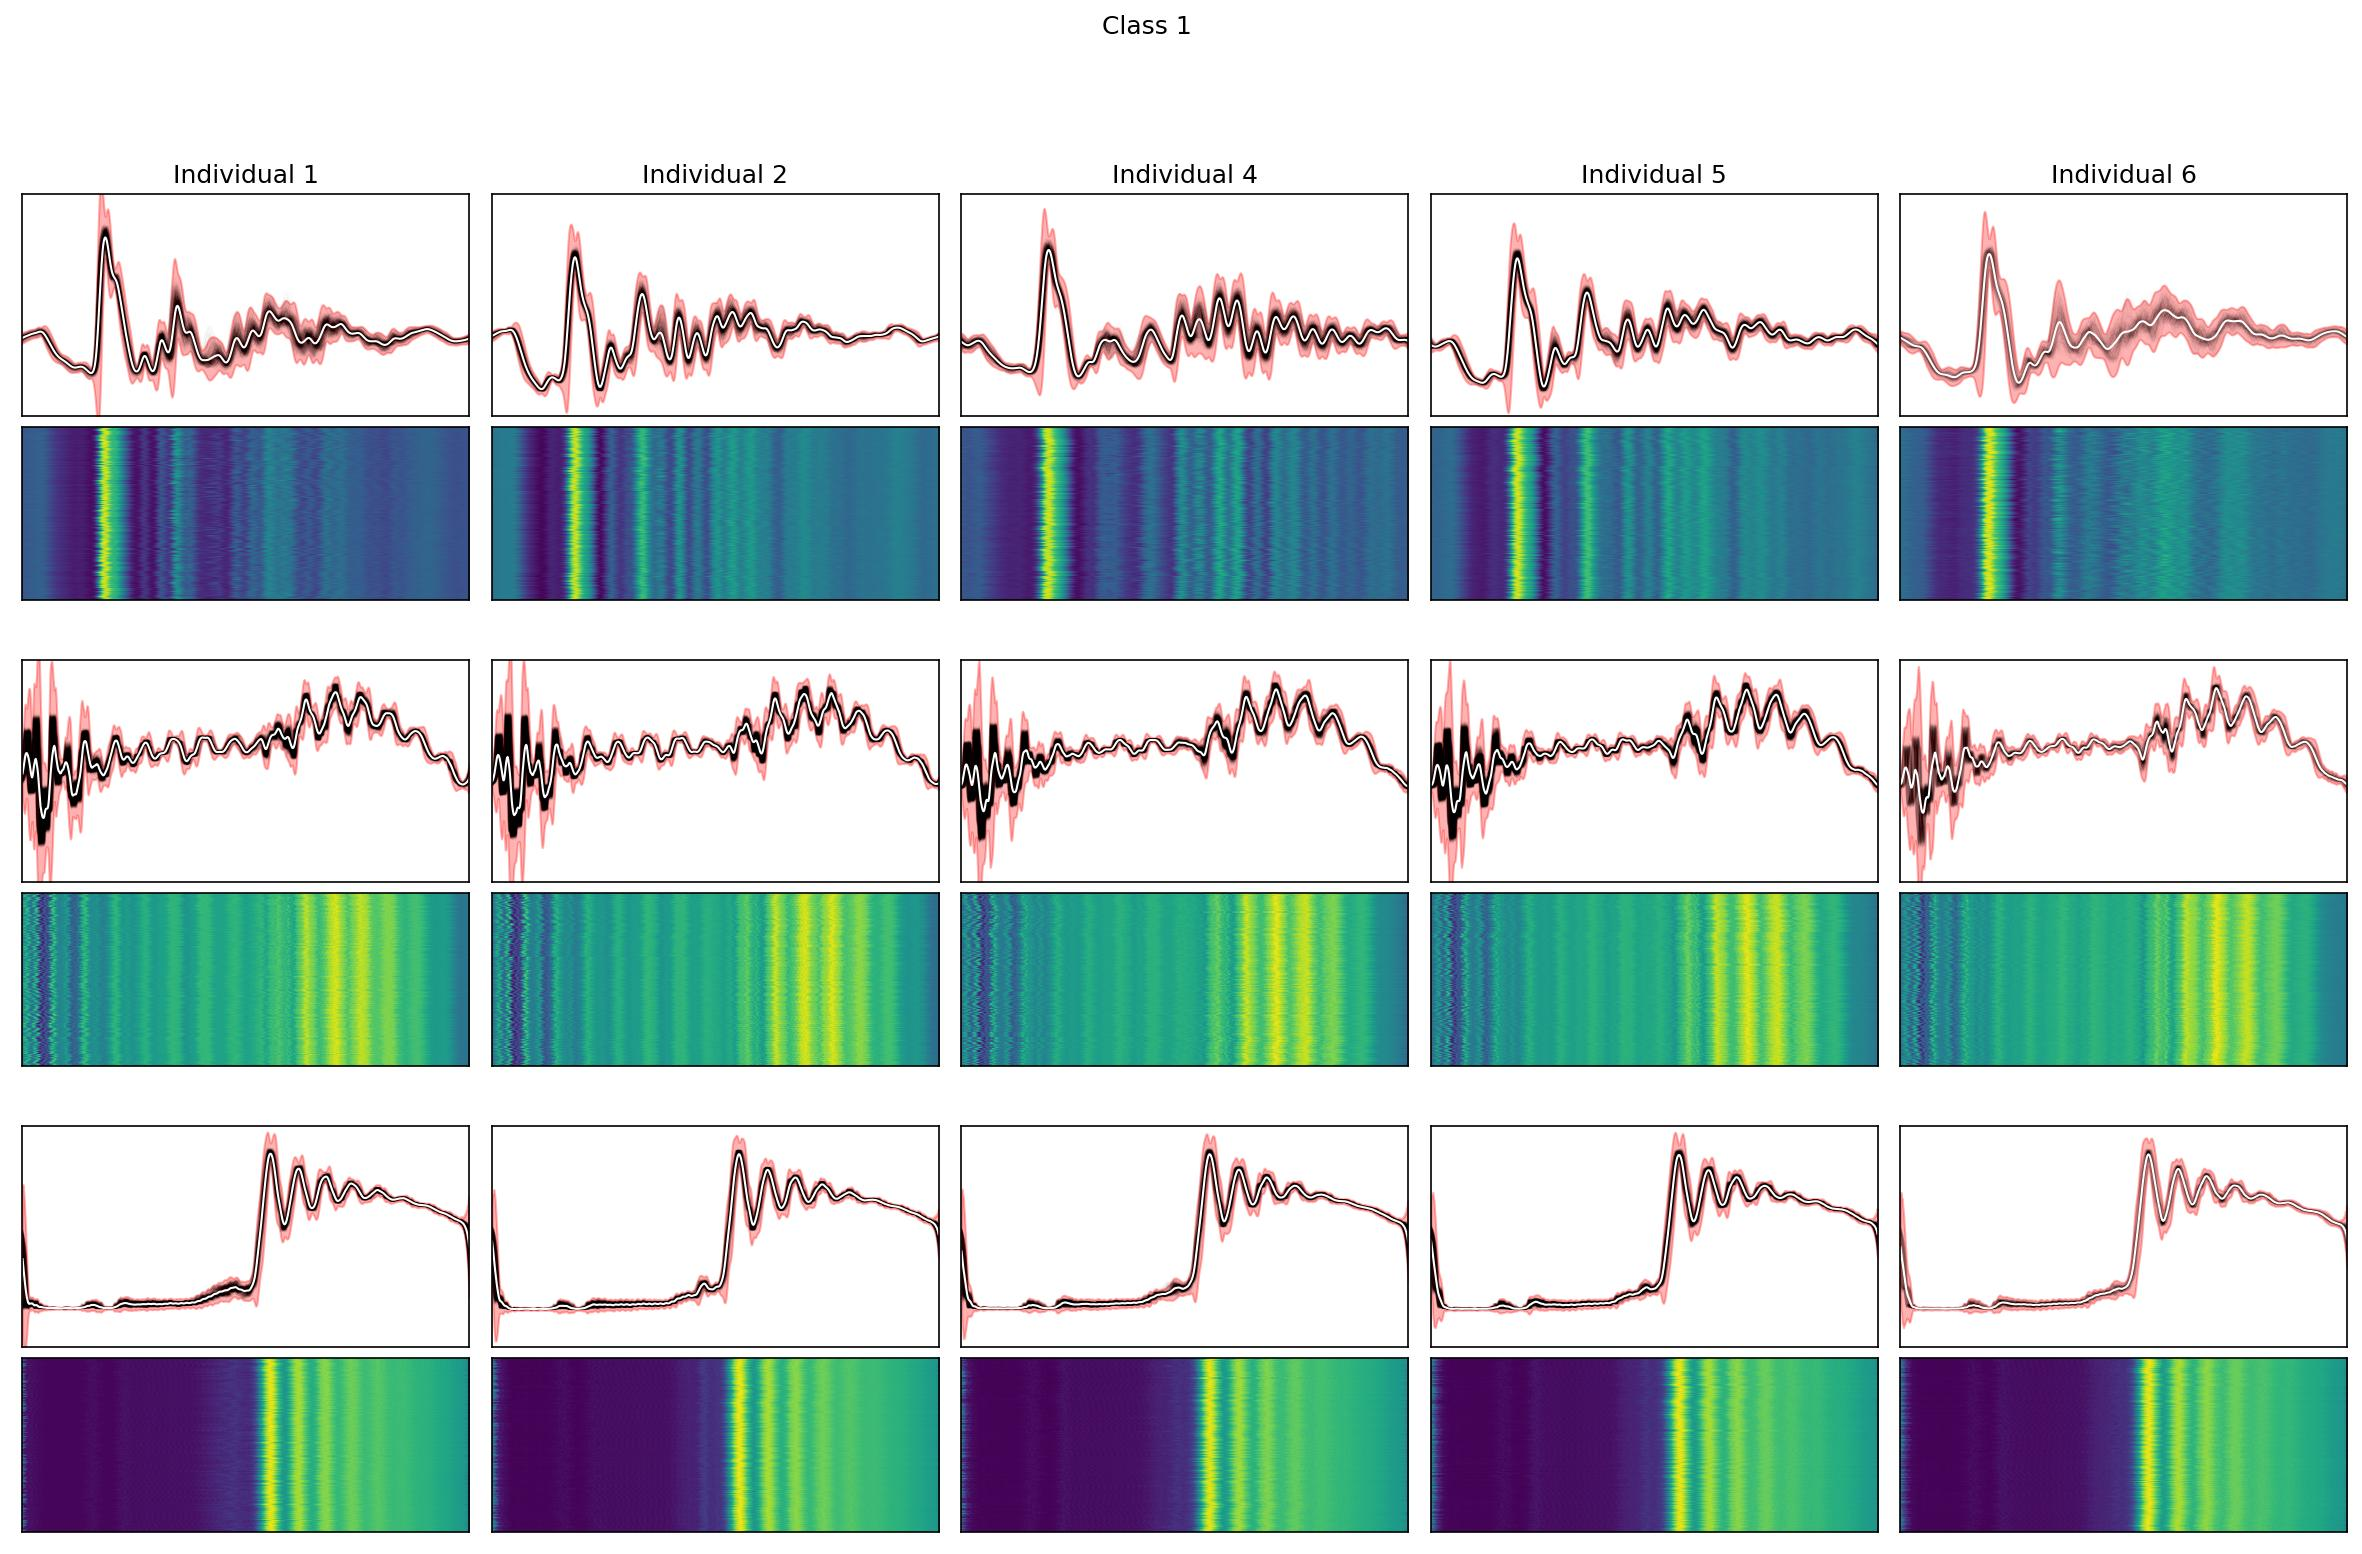
\includegraphics[width=\linewidth,trim=0 0 0 75,clip]{figures/original/plot_heatmap_class_1.jpg}
%         \caption{Original data (training set)}
%     \end{subfigure}
%     \vspace{0.5cm}
%     \begin{subfigure}{\linewidth}
%         \centering
%         % 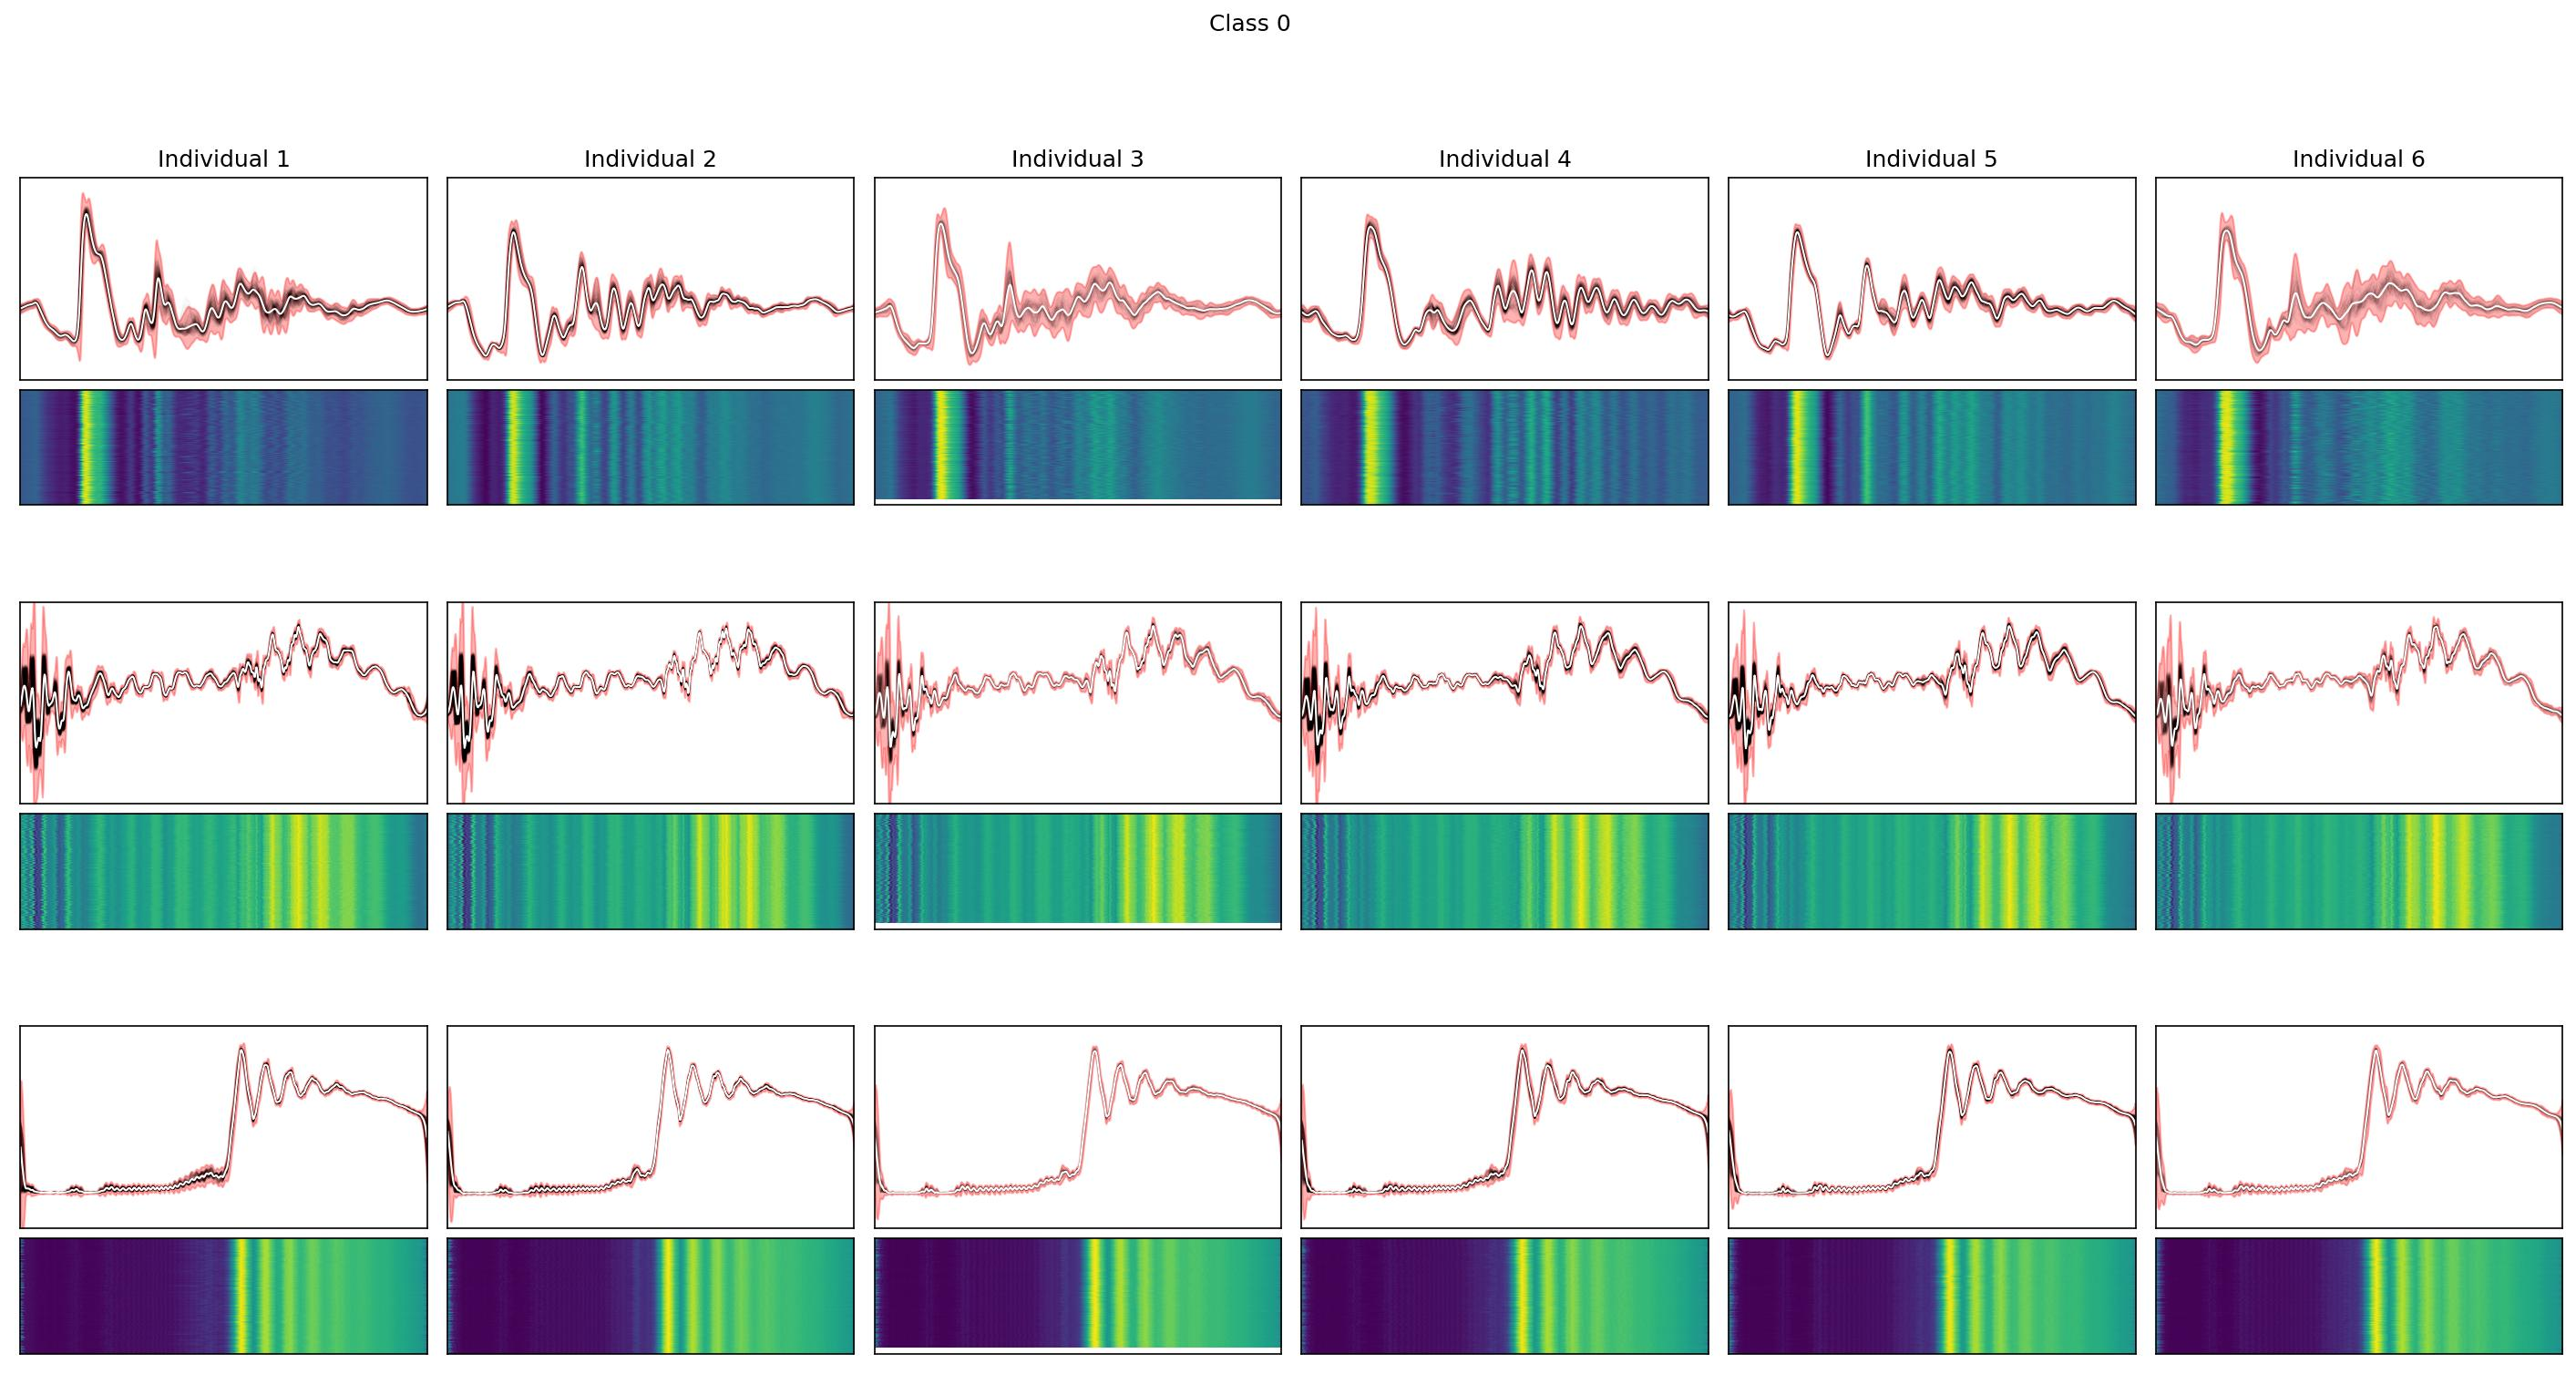
\includegraphics[width=\linewidth]{figures/aligned/plot_heatmap_class_1.jpg}
%         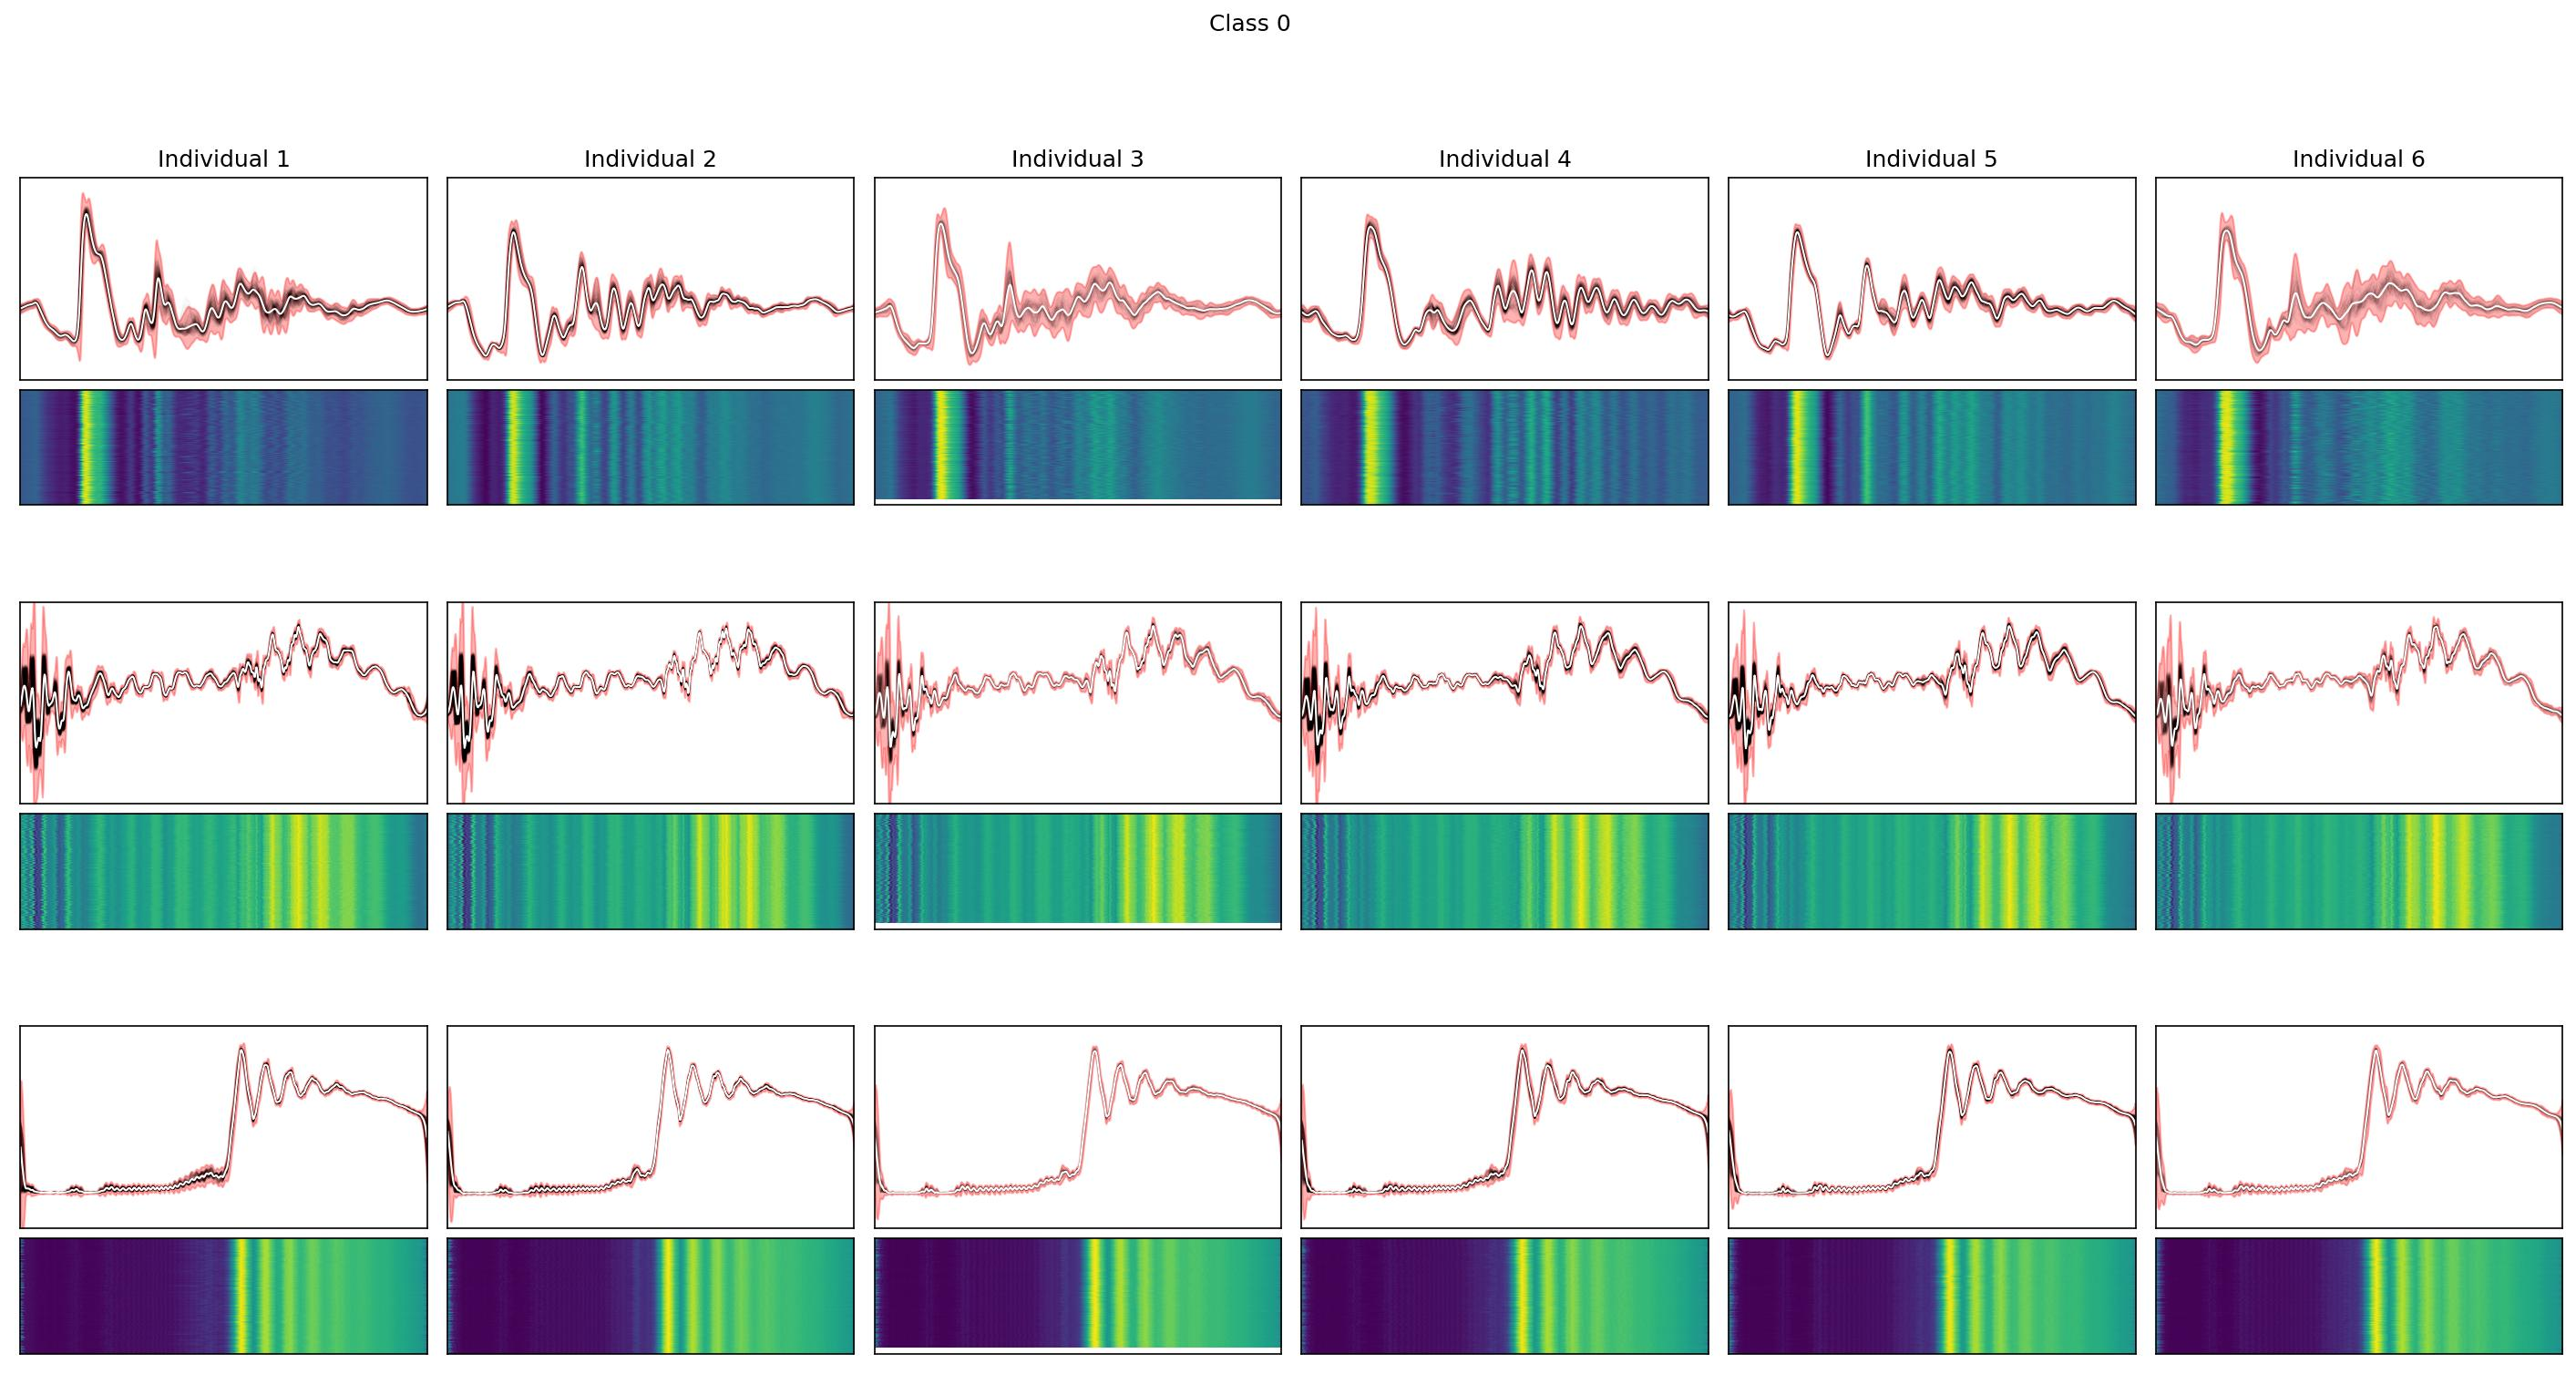
\includegraphics[height=0.57\linewidth,trim=0 0 905 75,clip]{figures/aligned/plot_heatmap_class_1.jpg}
%         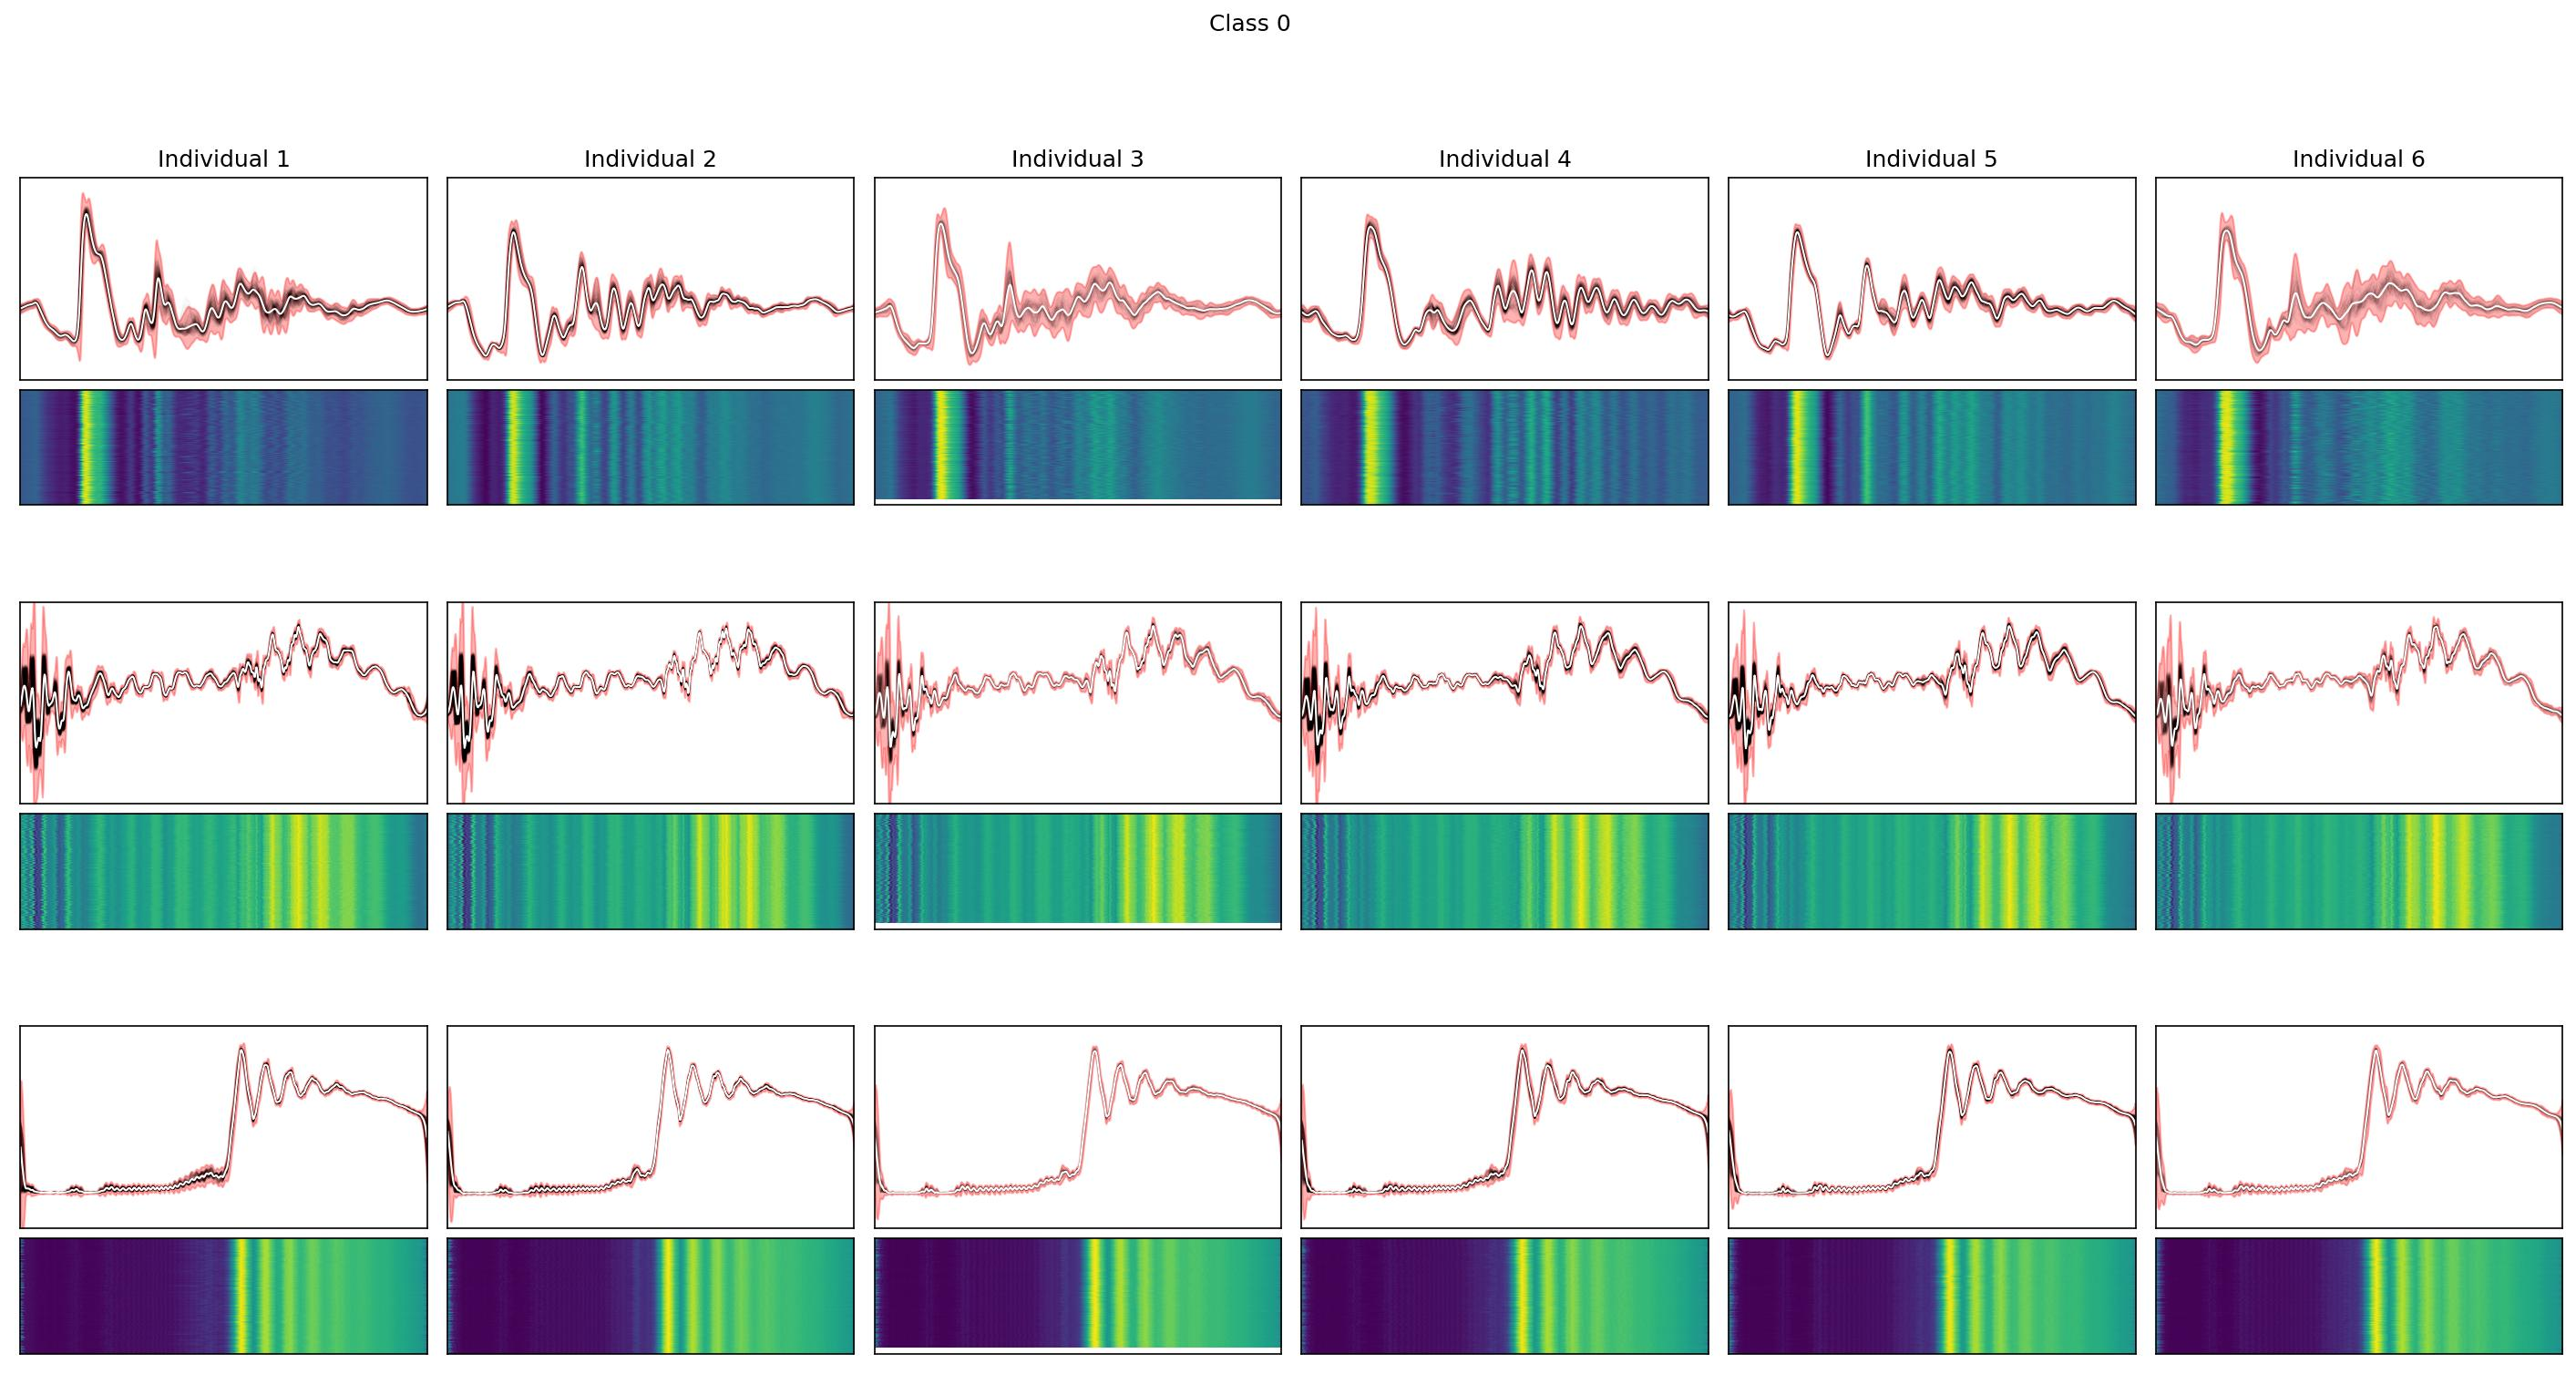
\includegraphics[height=0.57\linewidth,trim=685 0 0 75,clip]{figures/aligned/plot_heatmap_class_1.jpg}
%         \caption{Aligned data (test set)}
%     \end{subfigure}
%     \caption{Pressure sensor data before and after alignment: multiple individuals (1,2,4,5,6), and 3 channels (top: \textit{pin}, middle: \textit{pdin}, bottom: \textit{po})}
%     \label{fig:phm_alignment_2}
%     \end{center}
% \end{figure}

\clearpage
\section{Conclusions}\label{sec:conclusions_4}

% In this chapter, the methodological contributions on time series warping presented in \cref{chapter:2,chapter:3} were applied to the task of time series classification. 
The 2022 PHM Data Challenge provides an ideal opportunity to showcase the application of time series alignment in the specific area of fault diagnosis of a hydraulic rock drill using pressure data. 
Experiments have shown that accurate alignment leads to meaningful comparisons, reducing the risk of misinterpretation and misclassification. Hence, these results demonstrate the importance and effectiveness of aligning time series data for classification tasks. 
% Furthermore, the model has shown high accuracy in classifying faulty signals and has demonstrated its robustness to variability and complexity in real-world time series data.
The results also indicate that the reduction in variance seen in the training set is also present in the test and validation sets, indicating the model's ability to learn and generalize the warping functions present in the data to new samples. 


% In conclusion, time series classification has a wide range of applications and is a valuable tool in the analysis of sequential data. 
In conclusion, joining the flexibility of time series alignment methods with the potential of deep learning can improve the performance of time series classification. Our participation in the challenge resulted in a novel solution based on deep learning techniques that achieved an accuracy of 97.80\%, ranking sixth among the 18 competitors.

% The proposed model was submitted to the annual challenge organized by the Prognostics and Health Management Society, and ranked 6th out of 18 participants.

% In conclusion, the application of alignment methods for time series classification has been shown to be an effective approach in improving the accuracy and robustness of models. 


% ############################################################### END
